\section{正弦波の表式と縦波}

% ===========================================================================
%  再編（2026-09-04）：第2章 波動 の第14回．
%  原本の 第19回「正弦波の表式」の全体（19.1〜19.5）と，第20回「波動の干渉」の
%  冒頭 20.1「縦波」を1回に統合した．
%  ・練習は 原本 第19回［1］〜［8］（＝新［1］〜［6］［8］［9］）と
%    原本 第20回［10］縦波の横波表示（＝新［7］），［14］縦波と媒質の関係（＝新［10］）の10題．
%    `saihen/再編案.md` の「新14 ＝ ⑲[1]〜[8] ＋ ⑳[10][14]」の通り．
%  ・さらに 原本 第20回［9］の(1)(2)（縦波の横波表示の基本確認）を，新［1］の(5)(6)として
%    第15回から移した（2026-09-04 ユーザー指示）。この回で 14.6 縦波 を扱うため。
%    → 第15回では 原本［9］の (3)(4)(5) だけを ㉑［16］と統合すること。
%  ・並べ替え：縦波の［7］を B問題の最後に置き，講義の 14.6 縦波 と対応させた．
%    C問題は 波動の表式［8］→ 波の位相［9］→ 縦波と媒質の関係［10］の順．
%  ・原本の誤植を3件訂正した（「同一変異」→「同一変位」，「中心とすに」→「中心として」，
%    「波の伝搬方向」→「波の伝播方向」）．旧第20回のまとめ枠の見出しが「正弦波」に
%    なっていたのも内容に合わせて「横波と縦波」に改めた．
%  ・wrapfigure の [N] を図の実高（.xbb から算出）に合わせて付け直し，\bsNeed を追加した．
%
%  ・原本の例題5題をそのまま採用した（削除なし）。挿入位置も原本と同じ。
%      例題1〈正弦波〉                       … 14.1 のまとめ枠の後（原本 p86）
%      例題2〈正弦波の表式(1)〉               … 14.2 のまとめ枠の後（原本 p87）
%      例題3〈y-xグラフとy-tグラフの相互変換〉 … 14.3 の後（原本 p88）
%      例題4〈正弦波の表式(2)〉               … 14.4 のまとめ枠の後（原本 p89）
%      例題5〈縦波の横波表示〉                … 14.6 のまとめ枠の後（原本 p92）
%    波動（原本 第3章）の例題番号は章の先頭から1・2・3…（各章でリセット）で，
%    再編しても例題の順序は変わらないので原本の番号がそのまま使える。
%    原本は「問題枠 →（指針）＝空欄 →【KEY】」で解答が載っていないため，
%    【指針】と【解答】は書き起こした（KEY と問題文・図は原本からの転写）。
%    解答の図7枚は texify_draft/mkfig_new14ans.py（TikZ）で自作した。
% ===========================================================================

% 例題番号：波動（原本 第3章）の例題は章の先頭から1・2・3…（各章でリセット）
\setcounter{nombre}{0}

\bsNeed{30mm}   %% 図31.5mm ＋ 見出し14mm
\subsection{波長・周期・振動数・波の速さ}
\begin{wrapfigure}[6]{r}[5mm]{80mm}
  \centering
  \vspace{-5mm}
  
\includegraphics[keepaspectratio,width=80mm]
  {text_p85_fig1.png}
\end{wrapfigure}
壁に糸の一端をくくりつけ，もう一端を手で持ち，壁から離れて上下に振ると，右図のように糸の各部分が上下に振動し，振動の様子が右側に伝播していく．
このように何かしらの物理量が空間的に伝播していく現象を{\bf 波動}，または単に{\bf 波}と呼び，波を伝える物質を{\bf 媒質}と呼ぶ．
媒質はその場で振動し，振動の方向が波の伝播方向と垂直な波を{\bf 横波}と呼び，伝播方向と平行な波を{\bf 縦波}と呼ぶ．
先ほどの例は糸が媒質となっている横波である．
まずは横波について考えていこう．

\bsNeed{88mm}
% [N] は実高103.3mm＝19行分だが，この段落の中に \[ \] の別行立て数式が2つあり，
% その分だけ parshape の行数を早く使い切って $v=f\lambda$ の式が図に重なる．2行足して[21]にした．
\begin{wrapfigure}[21]{r}[5mm]{90mm}
  \centering
  \vspace{-5mm}
  
\includegraphics[keepaspectratio,width=90mm]
  {text_p85_fig2.png}
\end{wrapfigure}
伝播していく波の形が三角関数（$\sin$カーブ）である波を{\bf 正弦波}と呼ぶ．
伝播方向を$x$軸と設定し，ある時刻における$x$軸上の各点の変位を$y$[m]で表した$y-x$グラフは右図の実線のように表現できる．
$\sin$カーブ1つ分の長さを{\bf 波長}と呼び，変位の最大の大きさを{\bf 振幅}と呼ぶ．

各媒質は単振動をしていて，この単振動の周期と波の形が元の形に戻るまでの周期は一致する．
各媒質が単位時間あたりに何回振動するかを{\bf 振動数}と呼び，単位は{\bf [/s]=[Hz]（ヘルツ）}で表す．
周期を$T$[s]とすれば，振動数$f$[Hz]と$T$の間には
\[\mbox{\boldmath $f=\dfrac{1}{T}$}\]
が成立する．
また，波長を$\lambda$[m]とすれば，振動1回あたり$\lambda$[m]だけ波形が移動するので，波の伝播速度$v$[m/s]は
\[\mbox{\boldmath $v=f\lambda $}\]
となる．これを波の基本式という．

\begin{matome}{正弦波}
 \hspace{3mm} 正弦波：各質点が単振動をしており，$\sin$カーブの波形が伝わっていく波動\\
\hspace{3mm} 媒質：波動を伝える物質．その点で上下振動しているのみで，波形のみがずれていく．\\
% 波長の定義：「同一変位が現れる距離」だと y=A/2 の点が1波長に2つあるので誤解を招く
% （2026-09-05 修正）。同位相＝同じ振動状態、と言い切る。
\hspace{3mm} 波長：ある瞬間の波形において，同位相（＝同じ振動状態）にある隣り合う2点の間隔．山から次の山までの距離．\\
\hspace{3mm} 周期：ある媒質の上下振動に着目したときに媒質が同じ状態に戻るまでの時間，もしくは波形が一波長分ずれるのに要する時間\\
\hspace{4mm} 波の伝播速度\hspace{5mm}$v=f\lambda$\hspace{2mm}[m/s] \hspace{10mm} 波の振動数\hspace{5mm} $f=\dfrac{1}{T}$\hspace{2mm}[Hz]
 \end{matome}

%%%%%% 1.2pt罫＋見出し（約12mm）と問題枠がページで分かれないよう，ユニットごと送る
\bsNeed{102mm}
%%%%%  例題1（14.1 のまとめ枠の直後）＝ 原本【例題1】〈正弦波〉（p86）  %%%%%%%%%%
% 問題文・図・（指針）・KEY は原本からの転写。原本には解答が載っていないので【解答】は書き起こした。
\begin{reidaiunit}
\begin{reidai}{正弦波}
\hspace{1zw}$x$軸の正の方向に伝わる正弦波がある．図は，縦軸に媒質の変位$y\U{m}$，横軸に位置を表わす座標$x\U{m}$をとり，時刻$t=0\U{s}$における変位を実線で，時刻$t=0.1\U{s}$における変位を破線で示したものであり，実線の山$\mathrm{P}$は$0.1\U{s}$後に破線の山$\mathrm{Q}$に移った．これらを元に以下の問に答えよ．
\begin{center}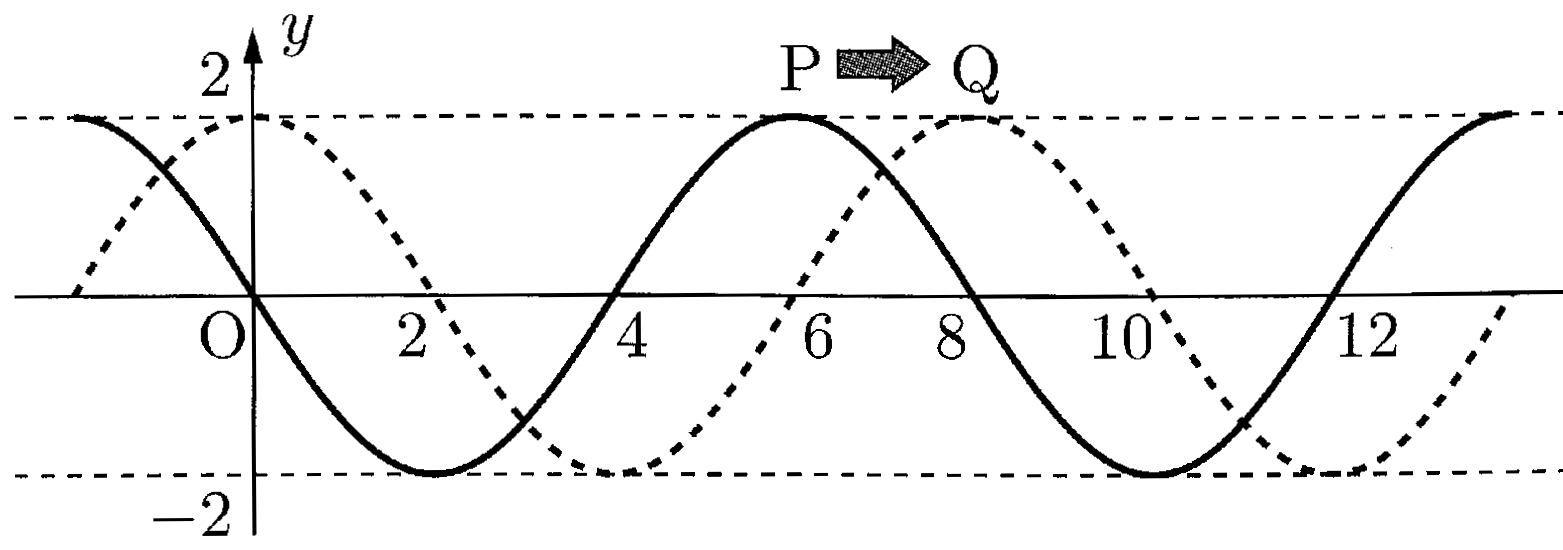
\includegraphics[keepaspectratio,width=110mm]{fig/n14_ex1_wave.png}\end{center}
\begin{komon}
\ko{1} この波の振幅$A\U{m}$，波長$\lambda\U{m}$，周期$T\U{s}$，振動数$f\U{Hz}$，速さ$v\U{m/s}$を求めよ．
\ko{2} 時刻$t=0\U{s}$において，$x=0$, $4$, $6\U{m}$の点はそれぞれどちら向きに動いているか．
\ko{3} 時刻$t=0\U{s}$において，媒質の速さが上向き最大である位置はどこか．$-2\leqq x\leqq 14\U{m}$の範囲について答えよ．
\ko{4} $t=1.4\U{s}$における波の波形を示せ．
\end{komon}
\end{reidai}

\begin{sisinE}
(2)(3) 媒質の移動を把握するためには次の瞬間の波の波形を書き，媒質各点の移動を押さえればよい．
\end{sisinE}
\Key{波長は「ある瞬間の波形で山から次の山までの間隔（＝同位相の隣り合う2点の間隔）」，周期は「媒質が同じ状態に戻るまでの時間」\quad $v=f\lambda$, $f=\dfrac{1}{T}$}

\begin{kaitou}
\begin{komon}
\ko{1} 実線の振れ幅より$A=2\U{m}$\Ans．また実線の波形は$x=0\U{m}$から$x=8\U{m}$までで1回繰り返しているから$\lambda=8\U{m}$\Ans．

       山$\mathrm{P}$（$x=6\U{m}$）が$0.1\U{s}$後に山$\mathrm{Q}$（$x=8\U{m}$）へ移ったのだから，波は$0.1\U{s}$の間に$2\U{m}$進んでいる．よって
       \[v=\frac{2}{0.1}=20\U{m/s}\Ans\]
       である．$v=f\lambda$と$f=\dfrac{1}{T}$より，
       \Ana{T=\frac{\lambda}{v}=\frac{8}{20}=0.40\U{s}\Ans,\hspace{5mm}f=\frac{1}{T}=2.5\U{Hz}\Ans}
\ko{2} 波は$+x$の向きに進むので，次の瞬間の波形は実線をわずかに右へずらしたものになる．{\gtfamily ある位置の媒質が上下どちらへ動くかは，その位置で「ずらした後の変位」が元より大きいか小さいかを見れば分かる}．

       $x=0\U{m}$：右へずらすと変位は正になるから，\AnaU{\gtfamily 上向き}\hspace*{\fill}\Ans

       $x=4\U{m}$：右へずらすと変位は負になるから，\AnaU{\gtfamily 下向き}\hspace*{\fill}\Ans

       $x=6\U{m}$：山の頂点（単振動の端点）にいるので，\AnaU{\gtfamily 動いていない（速度0）}\hspace*{\fill}\Ans
\ko{3} 媒質の速さが最大になるのは変位が0の点である．そのうち上向きに動くのは，(2)と同じ考え方で，波形を右へずらしたときに変位が正になる点，すなわち{\gtfamily 実線が右下がりに$x$軸を横切る点}である．$-2\leqq x\leqq 14\U{m}$では実線が$x$軸を横切るのは$x=0$, $4$, $8$, $12\U{m}$の4点で，このうち右下がりなのは$x=0\U{m}$と$x=8\U{m}$であるから，
       \Ana{x=0\U{m},\hspace{4mm}x=8\U{m}\Ans}
\ko{4} $t=1.4\U{s}$は$\dfrac{1.4}{0.40}=3.5$周期にあたる．波形は1周期で1波長ずれるから，$3.5$波長$=28\U{m}$だけ$+x$の向きにずれる．整数波長分のずれは波形を変えないので，これは半波長（$4\U{m}$）だけずれた波形と同じであり，$t=0\U{s}$の波形の正負を反転させたものになる．
       \begin{center}\AnaFig{110mm}{fig/n14_ex1_ans.png}{fig/n14_ex1_ans_blank.png}\end{center}
       \hspace{1zw}（実線が求める$t=1.4\U{s}$の波形，破線は$t=0\U{s}$の波形）\hspace*{\fill}\Ans
\end{komon}
\end{kaitou}
\end{reidaiunit}




\subsection{$y-x$グラフによる正弦波の一般式の導出}
ある波動の変位を式で表す場合には，どの場所の，いつの時刻の変位かの指定が必要であるから，波の変位$y$[m]は{\bf 位置} \mbox{\boldmath $x$}{\bf [m]と時刻}\mbox{\boldmath $t$} {\bf [s]の2変数関数}\mbox{\boldmath $y(x,t)$} {\bf[m]}となる．
そのため，この正弦波の方程式を直接立てることは非常に難しい．

そこで，正弦波の表式$y(x,t)$を得るには，まず片方の変数を固定したとき（通常は0とした場合）の表式を作り，その後，もう片方の変数を動かして，任意の$x,t$に対する変位を決定する．

どちらの変数を固定するかで2通りあるが，ここではまず，時刻$t$[s]を先に固定した場合を考える．
例えば時刻$t$[s]を$t=0$[s]に固定した場合，$y(x,0)$が表すものは時刻$t=0$[s]における波形である．
よって，与えられた時刻$t=0$[s]における波形グラフを具体的数式で表せば，$y(x,0)$が得られる．

\bsNeed{42mm}
\begin{wrapfigure}[10]{r}[5mm]{100mm}
  \centering
  \vspace{-5mm}
  
\includegraphics[keepaspectratio,width=100mm]
  {text_p87_fig1.png}
\end{wrapfigure}
この波が右方向に速さ$v$[m/s]で進んでいる場合について，任意の$t$[s]に対する変位$y(x,t)$を得ることを考えてみる．
時刻$t$[s]に位置$x$[m]にいる波は，時刻$t=0$[s]には距離$vt$[m]だけ手前の位置，すなわち$x-vt$[m]の場所にあったはずである．
よって，{\bf 時刻} \mbox{\boldmath $t$} {\bf [s]の位置} \mbox{\boldmath $x$} {\bf [m]の変位は，時刻} \mbox{\boldmath $t=0$} {\bf [s]の位置} \mbox{\boldmath $x-vt$} {\bf [m]の変位と一致していなければならない}から，
\[ \mbox{\boldmath $y(x,t)=y(x-vt,0)$}\]
が成立する．
すなわち，先ほど表した$y(x,0)$の式の$x$を$x-vt$に取り替えればよい．

利用できる波形のグラフが時刻$t=0$[s]のものでない場合や，波が左方向に進んでいる場合などはどのように置き換えるかはその都度考える必要があるが，その基本は，
\begin{matome}{波形グラフからの正弦波の一般表式の導出}
 \hspace{3mm} $\MARU{1} \hspace{2mm} 与えられたある時刻の波形グラフを数式で表す．（通常はt=0[{\rm s}]で考える）$\\
  \hspace{3mm} $\MARU{2} \hspace{2mm} 一般の時刻t[{\rm s}]における変位は，\MARU{1} の時刻ではどの位置にあったものかを計算する．$\\
   \hspace{3mm} $\MARU{3} \hspace{2mm} \MARU{2} を元に，y(x,t)を\MARU{1} の式から導く．右方向へ進むならy(x,t)=y(x-vt,0)$
 \end{matome}

%%%%%% 1.2pt罫＋見出し（約12mm）と問題枠がページで分かれないよう，ユニットごと送る
\bsNeed{42mm}
%%%%%  例題2（14.2 のまとめ枠の直後）＝ 原本【例題2】〈正弦波の表式\MARU{1}〉（p87）  %%%%%%%%%%
% 原本の（指針）欄は空欄。KEY は原本からの転写。指針と解答は書き起こした。
\begin{reidaiunit}
\begin{reidai}{正弦波の表式\MARU{1}}
\hspace{1zw}例題1の正弦波について以下の問に答えよ．
\begin{komon}
\ko{1} 時刻$t=0\U{s}$における波の変位$y(x,0)\U{m}$を表わす方程式を求めよ．
\ko{2} 任意の時刻$t\U{s}$，位置$x\U{m}$における波の変位$y(x,t)\U{m}$を表わす方程式を求めよ．
\end{komon}
\end{reidai}

\begin{sisinE}
まず(1)で$t=0\U{s}$の波形グラフを数式にする．振幅と波長さえ読み取れれば，$\sin$のカーブが原点からどちら向きに出ているかで符号が決まる．

(2)は公式を暗記して当てはめるのではなく，{\gtfamily 時刻$t\U{s}$に位置$x\U{m}$にある波が，$t=0\U{s}$にはどこにあったか}を毎回考える．例題1で$v=20\U{m/s}$と分かっているので，$20t\U{m}$だけ手前の位置にあったことになる．
\end{sisinE}
\Key{\MARU{1} $t=0\U{s}$の波形を数式化\quad \MARU{2} その時刻ではどの位置にあったかを計算\quad \MARU{3} 右向きに進む波なら$y(x,t)=y(x-vt,0)$}

\begin{kaitou}
\begin{komon}
\ko{1} $t=0\U{s}$の波形（実線）は，$x=0\U{m}$で$y=0\U{m}$であり，そこから$x$が増加すると変位が負になる正弦曲線である．振幅は$2\U{m}$，波長は$8\U{m}$であるから，
       \Ana{y(x,0)=-2\sin\left(2\pi\frac{x}{8}\right)=-2\sin\frac{\pi x}{4}\U{m}\Ans}
\ko{2} 波は$+x$の向きに速さ$20\U{m/s}$で進むので，時刻$t\U{s}$に位置$x\U{m}$にある波は，時刻$t=0\U{s}$には$x-20t\U{m}$の位置にあった．よって，
       \[y(x,t)=y(x-20t,\,0)=-2\sin\frac{\pi(x-20t)}{4}\]
       \Ana{=-2\sin 2\pi\left(\frac{x}{8}-\frac{t}{0.40}\right)\U{m}\Ans}
\end{komon}
\end{kaitou}
\end{reidaiunit}

である．


\subsection{$y-x$グラフと$y-t$グラフ}
波動の方程式は$x,t$の2変数関数であるから，ある波動の変位をグラフで表そうとした場合，どちらの変位を固定してグラフにするかでその方法は2通りある．
\begin{matome}{波動のグラフ化}
 \hspace{3mm} $・y-xグラフ$\\
  \hspace{5mm} ある瞬間における波の波形を，横軸に位置$x$[m]，縦軸に変位$y$[m]をとって表したグラフ\\
 \hspace{3mm} $・y-tグラフ$\\
  \hspace{5mm} ある1点の上下振動を，横軸に時間$t$[s]，縦軸に変位$y$[m]をとって表したグラフ
 \end{matome}

%%%%%% 1.2pt罫＋見出し（約12mm）と問題枠がページで分かれないよう，ユニットごと送る
\bsNeed{74mm}
%%%%%  例題3（14.3 の直後）＝ 原本【例題3】〈$y-x$グラフと$y-t$グラフの相互変換〉（p88）  %%%%%%%%%%
% 原本の（指針）欄は空欄。KEY は原本からの転写。指針と解答は書き起こした。
\begin{reidaiunit}
\begin{reidai}{$y-x$グラフと$y-t$グラフの相互変換}
\begin{zuright}{56mm}
\hspace{1zw}図の2つのグラフは，周期$T\U{s}$，速さ$v\U{m/s}$，振幅$A\U{m}$で$x$軸正の方向に進行している正弦波の，時刻$t=0\U{s}$における波形を示したものである．この2つの正弦波について，以下の設問に答えよ．
\begin{komon}
\ko{1} グラフの代表点に値を記入せよ．
\ko{2} 原点の振動を，時刻$t\U{s}$を横軸に，変位$y\U{m}$を縦軸に取ったグラフで表わせ．
\ko{3} 任意の時刻$t\U{s}$における原点の振動$y(0,t)\U{m}$を方程式で表わせ．
\end{komon}
\zusep
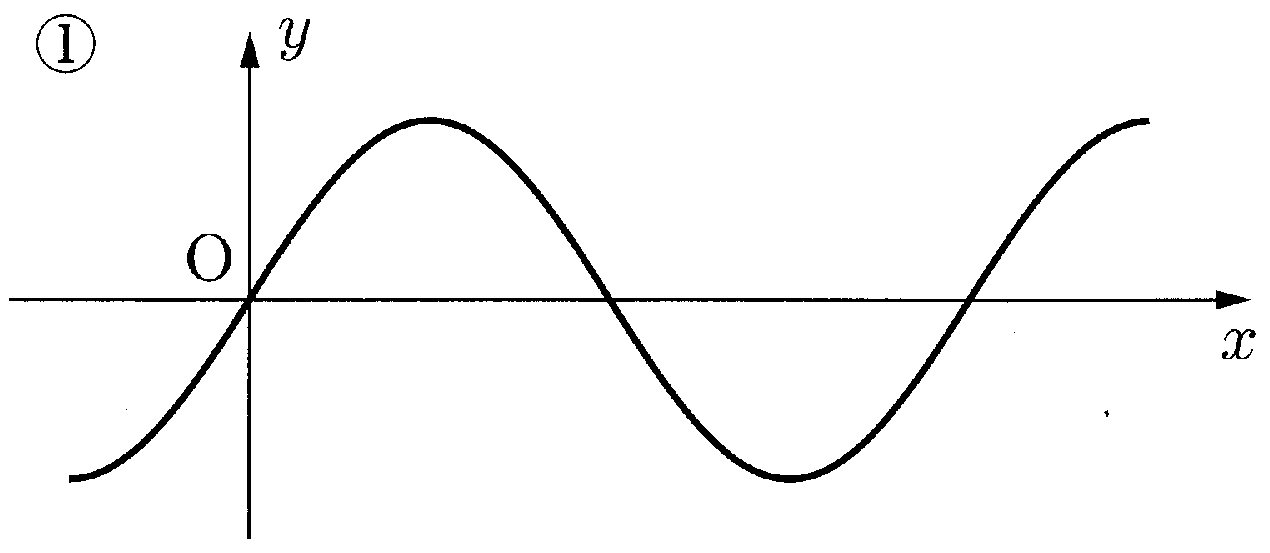
\includegraphics[keepaspectratio,width=54mm]{fig/n14_ex3_g1.png}\\[4mm]
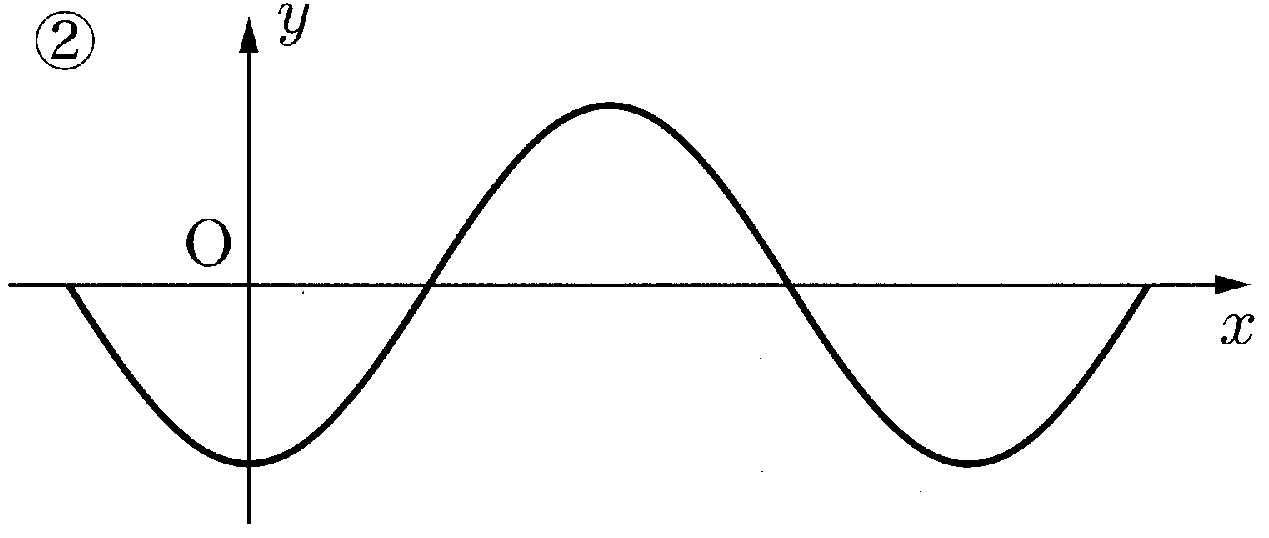
\includegraphics[keepaspectratio,width=54mm]{fig/n14_ex3_g2.png}
\end{zuright}
\end{reidai}

\begin{sisinE}
$y-x$グラフ（波形）と$y-t$グラフ（1点の振動）は，$\sin$カーブという見た目は同じでも意味がまったく違う．原点の$y-t$グラフを作るには，{\gtfamily 与えられた波形を少しだけ進行方向へずらしてみて，原点の媒質が上下どちらへ動き出すかを判定する}．

振幅$A\U{m}$・周期$T\U{s}$・$t=0\U{s}$での変位・動き出す向き，の4つが決まればグラフは1つに定まる．
\end{sisinE}
\Key{$y-x$グラフ$\rightarrow y-t$グラフの変換\quad$\Rightarrow$\quad{}波形を少し進めてみてどちらに動き出すかを把握}

\begin{kaitou}
\begin{komon}
\ko{1} 波長は$\lambda=vT\U{m}$であるから，$x$軸の代表点は$\dfrac{vT}{4}$, $\dfrac{vT}{2}$, $\dfrac{3vT}{4}$, $vT\U{m}$，$y$軸の代表点は$\pm A\U{m}$である．記入すると次のようになる．
       \begin{center}
       \begin{minipage}{82mm}\centering\MARU{1}\\[1mm]\AnaFig{78mm}{fig/n14_ex3_d1.png}{fig/n14_ex3_d1_blank.png}\end{minipage}\\[3mm]
       \begin{minipage}{82mm}\centering\MARU{2}\\[1mm]\AnaFig{78mm}{fig/n14_ex3_d2.png}{fig/n14_ex3_d2_blank.png}\end{minipage}
       \end{center}
       \hspace*{\fill}\Ans
\ko{2} いずれの波も$+x$の向きに進むので，次の瞬間の波形は右へわずかにずれる．

       \MARU{1}：原点は$y=0\U{m}$にあり，波形を右へずらすと変位は負になる．よって原点は$-y$の向きに動き出す．振幅$A\U{m}$，周期$T\U{s}$で，$t=0\U{s}$に$y=0\U{m}$から$-y$の向きに動き出す振動のグラフは次のものに限られる．

       \MARU{2}：原点は谷の底（$y=-A\U{m}$）にあり，単振動の端点であるから速度は0で，次の瞬間には変位が増加して$+y$の向きに動き出す．

       \begin{center}
       \begin{minipage}{82mm}\centering\MARU{1}\\[1mm]\AnaFig{78mm}{fig/n14_ex3_a1.png}{fig/n14_ex3_a1_blank.png}\end{minipage}\\[3mm]
       \begin{minipage}{82mm}\centering\MARU{2}\\[1mm]\AnaFig{78mm}{fig/n14_ex3_a2.png}{fig/n14_ex3_a2_blank.png}\end{minipage}
       \end{center}
       \hspace*{\fill}\Ans
\ko{3} (2)のグラフを数式化すると，
       \[\MARU{1}\hspace{3mm}y(0,t)=-A\sin\left(2\pi\frac{t}{T}\right)\U{m}\Ans\]
       \Ana{\MARU{2}\hspace{3mm}y(0,t)=-A\cos\left(2\pi\frac{t}{T}\right)\U{m}\Ans}
\end{komon}
\end{kaitou}
\end{reidaiunit}


いずれのグラフでも$\sin$カーブが現れるが，それらが意味するところは全く異なることに注意せよ．
またこれらのグラフは相互変換することができる．

\subsection{$y-t$グラフによる正弦波の一般式の導出}
ある瞬間における波形$y-x$グラフから正弦波の一般式を導出する方法を前々節で学んだが，問題文で与えられる波のグラフが，ある1点（通常は原点）の上下振動を$y-t$グラフとして表したものであることもしばしばある．
ここでは，与えられた$y-t$グラフから任意の時刻，位置における変位$y(x,t)$[m]を求める方法を学ぶ．
与えられた$y-t$グラフが原点$x=0$[m]における振動を表した$y-t$であり，波が右方向に速さ$v$[m/s]で進んでいる場合を考えよう．
まず，与えられた$y-t$グラフを具体的数式で表せば，$y(0,t)$[m]が得られる．

\bsNeed{42mm}
\begin{wrapfigure}[11]{r}[5mm]{100mm}
  \centering
  \vspace{-5mm}
  
\includegraphics[keepaspectratio,width=100mm]
  {text_p89_fig1.png}
\end{wrapfigure}
これを元に任意の$t$[s]に対する変位$y(x,t)$[m]を得るためには，時刻$t$[s]に位置$x$[m]にいる波が，原点をいつ通過したかを考えればよい．
位置$x$[m]に来るためには原点から$\dfrac{x}{v}$[s]だけかかるから，時刻$t$[s]に位置$x$[m]にある波は原点を$t-\dfrac{x}{v}$[s]に通過した波である．
よって，{\bf 時刻} \mbox{\boldmath $t$} {\bf [s]における位置} \mbox{\boldmath $x$} {\bf [m]の変位は，原点における時刻} \mbox{\boldmath $t-\dfrac{x}{v}$} {\bf [s]の変位と一致していなければならない}ので，
\[\mbox{\boldmath $y(x,t)=y\left( 0,t-\dfrac{x}{v}\right)$}\]
が成立する．
すなわち，先ほど表した$y(0,t)$の式の$t$を，$t-\dfrac{x}{v}$に取り替えれば$y(x,t)$が得られる．

利用できる$y-t$グラフが原点のものでない場合や，波が左方向に進んでいる場合などはどのように置き換えるかをその都度考える必要があるが，その基本は次の通りである．

\begin{matome}{振動グラフからの正弦波の一般表式の導出}
 \hspace{3mm} $\MARU{1} \hspace{2mm} 与えられたある点の振動グラフを数式で表す．（通常はx=0[{\rm m}]で考える）$\\
  \hspace{3mm} $\MARU{2} \hspace{2mm} 一般のx[{\rm m}]における変位は，\MARU{1} の点をどの時刻に通過したものかを計算する．$\\
   \hspace{3mm} $\MARU{3} \hspace{2mm} \MARU{2} を元に，y(x,t)を\MARU{1} の式から導く．右方向へ進むならy(x,t)=y\left(0,t-\dfrac{x}{v}\right)$
 \end{matome}

% 問題枠（約62mm）が入り切らないと，前ページに枠の下罫だけが残る．ユニットごと次ページへ送る．
\bsNeed{83mm}
%%%%%%%%%%  例題4（14.4 のまとめ枠の直後）＝ 原本【例題4】〈正弦波の表式\MARU{2}〉（p89）  %%%%%%%%%%
% 原本の（指針）欄は空欄。KEY は原本からの転写。指針と解答は書き起こした。
\begin{reidaiunit}
\begin{reidai}{正弦波の表式\MARU{2}}
\begin{zuright}{62mm}
\hspace{1zw}右図のグラフは，周期$T\U{s}$，速さ$v\U{m/s}$，振幅$A\U{m}$で$x$軸正の方向に進行している正弦波の原点の振動を，時刻$t\U{s}$を横軸に，変位$y\U{m}$を縦軸に取ったグラフとして表わしたものである．これについて以下の問に答えよ．
\begin{komon}
\ko{1} グラフの$t$, $y$座標の代表点に値を記入せよ．
\ko{2} (1)を元に，原点における波の変位$y(0,t)\U{m}$を方程式で表わせ．
\ko{3} 任意の時刻$t\U{s}$，位置$x\U{m}$における波の変位$y(x,t)\U{m}$を表わす方程式を求めよ．
\ko{4} 波が$x$軸負の方向に同じ速さで進んでいる場合，波の変位$y(x,t)\U{m}$はどうなるか，その方程式を求めよ．
\end{komon}
\zusep
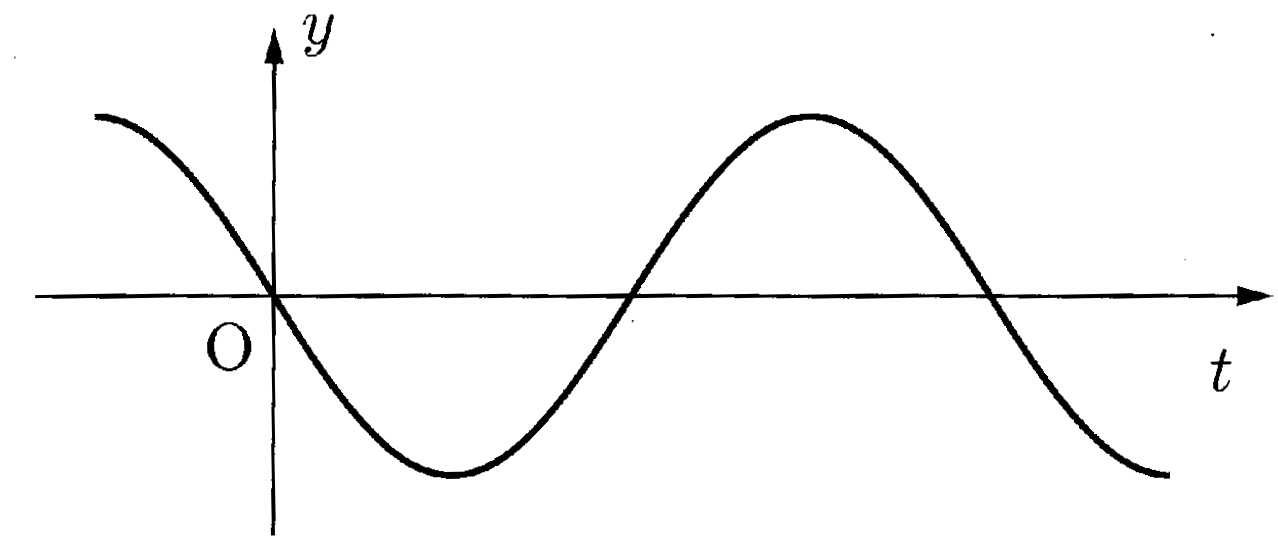
\includegraphics[keepaspectratio,width=62mm]{fig/n14_ex4_yt.png}
\end{zuright}
\end{reidai}

\begin{sisinE}
与えられているのは{\gtfamily 波形ではなく原点の振動}である．横軸が$t$であることを見落とさないこと．

一般表式を得るには，{\gtfamily 時刻$t\U{s}$に位置$x\U{m}$にある波が，原点をいつ通過したか}を考える．$+x$の向きに進む波なら，原点から$x\U{m}$進むのに$\dfrac{x}{v}\U{s}$かかるので，通過時刻は$t-\dfrac{x}{v}\U{s}$である．(4)は波の進む向きが逆になるので，位置$x\U{m}$の波はまだ原点を通過しておらず，これから通過する．そのため通過時刻は$t+\dfrac{x}{v}\U{s}$となり，符号が変わる．
\end{sisinE}
\Key{\MARU{1} 原点の$y-t$グラフを数式化\quad \MARU{2} その点をどの時刻に通過したかを計算\quad \MARU{3} 右向きに進む波なら$y(x,t)=y\left(0,\,t-\dfrac{x}{v}\right)$}

\begin{kaitou}
\begin{komon}
\ko{1} 原点の単振動の周期は波の周期$T\U{s}$に，振幅は波の振幅$A\U{m}$に一致するから，代表点は次のように記入できる．
       \begin{center}\AnaFig{76mm}{fig/n14_ex4_ans.png}{fig/n14_ex4_ans_blank.png}\end{center}
       \hspace*{\fill}\Ans
\ko{2} $t=0\U{s}$で$y=0\U{m}$であり，そこから変位が負になっていくので，
       \Ana{y(0,t)=-A\sin\left(2\pi\frac{t}{T}\right)\U{m}\Ans}
\ko{3} 波は$+x$の向きに速さ$v\U{m/s}$で進むので，時刻$t\U{s}$に位置$x\U{m}$にある波が原点を通過したのは時刻$t-\dfrac{x}{v}\U{s}$である．よって，
       \[y(x,t)=y\left(0,\,t-\frac{x}{v}\right)=-A\sin\left\{2\pi\frac{t-x/v}{T}\right\}\]
       \Ana{=-A\sin 2\pi\left(\frac{t}{T}-\frac{x}{vT}\right)\U{m}\Ans}
\ko{4} 波が$-x$の向きに進む場合は，時刻$t\U{s}$に位置$x\U{m}$にある波が原点を通過するのは時刻$t+\dfrac{x}{v}\U{s}$である（原点はまだ通過していない）．よって，
       \Ana{y(x,t)=y\left(0,\,t+\frac{x}{v}\right)=-A\sin 2\pi\left(\frac{t}{T}+\frac{x}{vT}\right)\U{m}\Ans}
\end{komon}
\end{kaitou}
\end{reidaiunit}


\subsection{正弦波の一般式の一般形}
以上で求めてきた正弦波の任意の時刻，任意の位置の変位$y(x,t)$[m]は必ず
\[ y(x,t)=A\sin \left\{ 2\pi \left( \dfrac{t}{T}\pm \dfrac{x}{\lambda} \right) +\varphi_0 \right\}  \hspace{5mm} (A,\varphi_0 は定数) \]
の形にまとめることができる．
この式を覚えておく必要はないが，正弦波がグラフではなく数式で与えられた場合はこの三角関数の中身の部分に着目して考えるとよい．

三角関数の角度部分を{\bf 位相}と呼ぶ．
\[\varphi (x,t)=2\pi \left( \dfrac{t}{T}\pm \dfrac{x}{\lambda} \right) +\varphi_0\]

この位相が同じ値であれば変位$y(x,t)$は同じになる．
ゆえに，波が進行していくということは同一位相の点が右もしくは左へずれていくということを意味する．

% 加筆（2026-09-14 ユーザー指摘）：ここは「これより」の一言で結論に飛んでおり，
%   位相を一定に保って x を t で表す一段が無いと，生徒は結論を丸暗記するしかなかった。
\hspace{1zw}実際，異符号の場合について位相を一定の値に保つと
\[2\pi \left( \dfrac{t}{T}-\dfrac{x}{\lambda} \right)+\varphi_0=\text{（一定）}
  \hspace{5mm}\Longleftrightarrow\hspace{5mm} x=\dfrac{\lambda}{T}t+\text{（定数）}\]
となり，時刻$t$[s]が増えるとその位相をもつ位置$x$[m]も増えていく．
すなわち同一位相の点が右へ移動する．同符号の場合は同じ計算で$x=-\dfrac{\lambda}{T}t+$（定数）となり，左へ移動する．
なお$\dfrac{\lambda}{T}$はこの点の移動する速さであり，$v=\dfrac{\lambda}{T}=f\lambda$と一致している．

\hspace{1zw}これより，位相部分の$x,t$の係数が{\bf 異符号であれば波は右方向へ，同符号であれば波は左方向へ進行する}ということが言える．

また，位相は$2\pi$ずれても同じ変位になることに注意すると，ある時刻$t$[s]において位置$x$[m]が$\lambda$[m]だけずれると位相が$2\pi$だけずれるので同一変位となる．
よって，同一時刻において位置のずれを位相のずれに換算するなら，{\bf 1波長のずれが位相} \mbox{\boldmath $2\pi$} {\bf のずれに対応する．}

またある位置において時刻$t$[s]が変化していくと，時刻が$T$[s]だけずれると位相が$2\pi$だけずれて再び同一変位となる．よって，ある位置において時刻のずれを位相のずれに換算するなら，{\bf 1周期}\mbox{\boldmath $T$}{\bf [s]のずれが位相} \mbox{\boldmath $2\pi$}{\bf のずれに対応する．}

また，{\bf 位相が}\mbox{\boldmath $\pi$}{\bf ずれているとその変位がちょうど正負逆}となる．
このような2つの位相を{\bf 互いに逆位相である}という．
\begin{matome}{正弦波のまとめ}
 \hspace{3mm} $・三角関数の角度の部分を位相と呼ぶ．この位相が2\pi ずれても同じ変位になる．$\\
 \hspace{3mm} $・位相部分のx，tが異符号なら右方向へ，同符号なら左方向へ進行する波である．$\\
 \hspace{3mm} $・ある時刻において，位置が\lambda [{\rm m}]ずれると位相は2\pi ずれる．$\\ 
 \hspace{3mm} $・ある位置において，時刻がT[{\rm s}]ずれると位相は2\pi ずれる．$\\ 
 \hspace{3mm} $・位相が\pi ずれると変位は上下逆となる．$\end{matome}



% wfcheck.py はこの \bsNeed を「図の直前に無い」と指摘するが，これは誤検出．
% チェックリストの通り \subsection の「前」に置いてある（後ろに置くと見出しだけが前ページに残る）．
\bsNeed{92mm}  %% 見出し14mm ＋ 導入2行11mm ＋ 図76.1mm−9mm
\subsection{縦波}
弦の振動のように，波の進行方向に対して垂直な方向に媒質が振動する波を{\bf 横波}と呼ぶ．
波にはこの横波の他に，波の進行方向と平行に媒質が振動する波である{\bf 縦波}がある．

% 原本は幅120mm（実高101.5mm）だが，本文の段が35mmしか残らず読みにくいうえ，
% ページ下端からはみ出しやすい．90mm（実高76.1mm＝14行分）に縮めた．
\begin{wrapfigure}[14]{r}[5mm]{90mm}
  \centering
  \vspace{-5mm}
  
\includegraphics[keepaspectratio,width=90mm]
  {text_p91_fig1.png}
\end{wrapfigure}
縦波を理解するためには図のような等しい質量をもつ小球と等しいバネとが連結されて水平面上に置かれている状況を考えるとよい．

この図において，一番左端の小球$P_0$を左右に単振動させると，$P_0$の振動につられて$P_1$が動き出し，それにつられて$P_2$が，というように$P_0$の振動が右方向に順に伝わっていく．
$P_0$の単振動が右端に達して左に戻ると，それにつられて$P_1$も左へ，$P_2$も，というように振動するため，各小球は初期位置を中心として波の進行方向と平行な方向に振動する．
このように，{\bf 媒質の振動方向と平行に振動が伝播する波のことを縦波という．}

各小球は少しずつ時間がずれて単振動するため，小球が集まって密度が高くなる部分（密部）と，小球が離れて密度が低くなる部分（疎部）とができ，これらの密部，疎部が波の進行方向へ一定の速さで伝播していく．
そのため，縦波は疎密波と呼ばれることもある．

\bsNeed{53mm}
\begin{wrapfigure}[13]{r}[5mm]{60mm}
  \centering
  \vspace{-5mm}
  
\includegraphics[keepaspectratio,width=60mm]
  {text_p91_fig2.png}
\end{wrapfigure}
縦波の各点の振動は波の伝播方向と一致しているため，そのまま図示すると分かりにくい．
そこで，振動中心からの変位を縦軸にしたグラフを用いることが多い．
この際，{\bf 媒質の変位は初期位置からの変位を反時計回りに90度回転させて図示すればよい．}
媒質が$x$軸正の向きに変位したときに，$y$軸正の向きに変位を取るようにして図示するとちょうど横波と同様な$y-x$グラフとなるため，数式的には横波と同様にして扱うことができる．
これを{\bf 縦波の横波表示}という．
横波表示された縦波の媒質の各点の変位を実際の変位に戻すためには，$y$軸正の向きの変位を時計回りに90度回転させて，$x$軸正の向きの変位に直せばよい．

% 加筆（2026-09-10）：疎密の判定は例題5とその注，練習［10］の解答で言葉としては述べているが，
% 「グラフの傾き」という形の規則になっていなかった。第16回 16.4（気柱の例題）の指針が
% 「横波表示のグラフの傾きが疎密を表すこと」を既知として参照しているため，ここで規則化する。
縦波では，媒質が最も集まっている点（密）と最も離れている点（疎）がどこかを問われることが多い．
横波表示のグラフからこれを読み取るには，{\gtfamily 注目する点の両側の媒質が，その点に近づく向きに変位しているか，遠ざかる向きに変位しているかを見ればよい}．
変位が$0$の点のうち，$x$の増加とともに変位が正から負へ変わる点（グラフの傾きが負の点）では，左側の媒質が$x$軸正の向きに，右側の媒質が$x$軸負の向きに変位しているから，媒質は互いに近づいており{\gtfamily 密}である．
逆に，負から正へ変わる点（グラフの傾きが正の点）では媒質は互いに遠ざかっており{\gtfamily 疎}である．

\begin{matome}{横波と縦波}
 \hspace{3mm} 横波：波の進行方向と媒質の変位方向が垂直であるもの．水面波，弦の振動など．\\
\hspace{3mm} 縦波：波の進行方向と媒質の変位方向が平行であるもの．疎密波とも呼ばれる．音波など．\\[1mm]
\hspace{3mm} 縦波の疎密の判定（横波表示のグラフの変位$0$の点で）\\
\hspace{5mm} $\Rightarrow$\quad{}$x$の増加とともに変位が正から負へ変わる点（傾きが負）\ $\cdots$\ {\gtfamily 密}\\
\hspace{5mm} \phantom{$\Rightarrow$}\quad{}$x$の増加とともに変位が負から正へ変わる点（傾きが正）\ $\cdots$\ {\gtfamily 疎}
 \end{matome}

%%%%%% 1.2pt罫＋見出し（約12mm）と問題枠がページで分かれないよう，ユニットごと送る
\bsNeed{83mm}
%%%%%  例題5（14.6 のまとめ枠の直後）＝ 原本【例題5】〈縦波の横波表示〉（p92）  %%%%%%%%%%
% 原本の（指針）欄は空欄。KEY は原本からの転写。指針と解答は書き起こした。
% 横軸の単位（2026-09-14 補筆。もとは TODO だった）：原本の図の横軸には単位の表記が無いが，
%   [m] として扱わないと解答の λ=20[m]・v=4.0×10^2[m/s] が決まらない。問題文に
%   「横軸の目盛の単位は[m]」を明記した（原本にない補筆）。
%   あわせて，原本の図は A〜E に点も垂線も打っておらず B・D が x=10・20 なのかを
%   読み取りにくいので，解答の冒頭で 5 点の位置を確定させてある（ユーザー指摘）。
\begin{reidaiunit}
\begin{reidai}{縦波の横波表示}
\begin{zuright}{68mm}
\hspace{1zw}右図は$x$軸上を正の向きに伝わる縦波の時刻$t=0\U{s}$のときの様子を，媒質の振動中心の位置を横軸に，媒質変位を縦軸にとって示したものである．この波の振動数を$f=20\U{Hz}$とし，図の横軸の目盛の単位は$\U{m}$として，以下の問に答えよ．
\begin{komon}
\ko{1} この波の波長と波の速さを求めよ．
\ko{2} 時刻$t=0\U{s}$のとき，図の$\mathrm{A}$, $\mathrm{B}$, $\mathrm{C}$, $\mathrm{D}$, $\mathrm{E}$の各点において，最も疎な点はどこか．
\ko{3} 時刻$t=0\U{s}$のとき，媒質の振動の向きが波の進む向きと逆向きでその速さが最大になる点は$\mathrm{A}$, $\mathrm{B}$, $\mathrm{C}$, $\mathrm{D}$, $\mathrm{E}$のうちどれか．
\end{komon}
\zusep
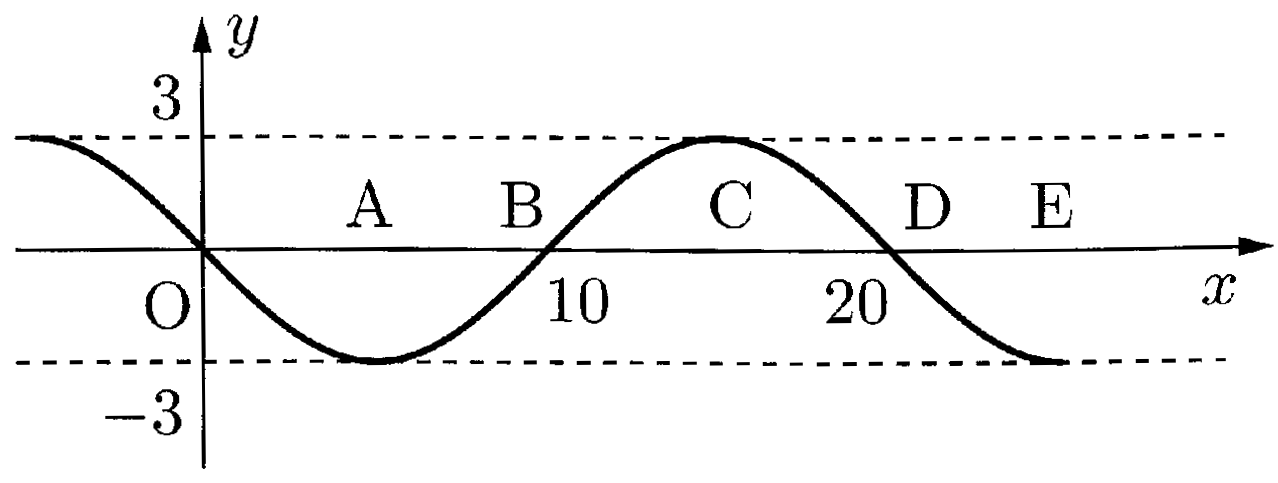
\includegraphics[keepaspectratio,width=68mm]{fig/n14_ex5_long.png}
\end{zuright}
\end{reidai}

\begin{sisinE}
横波表示のグラフをそのまま眺めても疎密は判定できない．{\gtfamily $+y$の向きの変位を$+x$の向きの変位に戻し，媒質が実際にどこへ動いたかを図示する}こと．周りから媒質が集まってくる点が密，遠ざかっていく点が疎である．

(3)の媒質の速度は，横波と同じように{\gtfamily 次の瞬間の波形（右へわずかにずらしたもの）}を描いて判定し，最後に$\pm y$を$\pm x$に読み替える．
\end{sisinE}
\Key{疎密点の判断\quad$\Rightarrow$\quad{}媒質の変位を元に戻して考える}

\begin{kaitou}
\hspace{1zw}まず図から各点の位置を読み取ると，$\mathrm{A}$, $\mathrm{B}$, $\mathrm{C}$, $\mathrm{D}$, $\mathrm{E}$はそれぞれ$x=5, 10, 15, 20, 25\U{m}$の点である（$\mathrm{A}$と$\mathrm{E}$が谷，$\mathrm{C}$が山，$\mathrm{B}$と$\mathrm{D}$が変位0の点）．
\begin{komon}
\ko{1} グラフより，波形は$x=0\U{m}$から$x=20\U{m}$までで1回繰り返しているから，
       \[\lambda=20\U{m}\Ans\]
       である．よって波の速さは，
       \Ana{v=f\lambda=20\times 20=4.0\times 10^{2}\U{m/s}\Ans}
\ko{2} 横波表示の変位を実際の（$x$方向の）変位に戻して媒質の位置を図示すると，次のようになる．
       \begin{center}\AnaFig{100mm}{fig/n14_ex5_ans.png}{fig/n14_ex5_ans_blank.png}\end{center}
       \hspace{1zw}（上段が振動中心の位置，下段が実際の媒質の位置）

       $\mathrm{B}$の付近では媒質が左右へ遠ざかり，$\mathrm{D}$の付近では媒質が左右から集まっている．よって最も疎な点は，
       \[\mathrm{B}\Ans\]
\ko{3} 媒質の速さが最大になるのは変位が0の点，すなわち$\mathrm{B}$と$\mathrm{D}$である．波は$+x$の向きに進むので，次の瞬間の横波表示の波形は右へわずかにずれる．すると$\mathrm{B}$の変位は負に，$\mathrm{D}$の変位は正になる．

       このグラフは{\gtfamily $+x$の向きの変位を$+y$の向きに取り直した}ものだから，横波表示で$y$が減少することは，実際には媒質が$-x$の向きへ動くことを意味する．よって$\mathrm{B}$の媒質は$-x$の向きに，$\mathrm{D}$の媒質は$+x$の向きに動く．波の進む向きは$+x$であるから，求める点は，
       \Ana{\mathrm{B}\Ans}
\end{komon}
\end{kaitou}
\begin{chuu}
(2)と(3)の答えが一致したのは偶然ではない．疎になる点では媒質が左右へ遠ざかっており，その中心の媒質は波の進行と逆向きに最も速く動いている．逆に密になる点（本問では$\mathrm{D}$）では，媒質は波の進行と同じ向きに最も速く動いている．
\end{chuu}
\end{reidaiunit}


% ===========================================================================
%  14.7・14.8 を加筆した（2026-09-10）。
%  ・14.7 は physics_new18.tex の 18.3 前半（波面／ホイヘンスの原理／回折）を
%    図3枚ごと移設したもの。波面・ホイヘンス・回折は波動一般の性質であり，
%    第18回（光）で初めて登場するのは提示順序が逆だったため（ChatGPT指摘・裏取り済み）。
%    移設に伴い，第18回 18.4 は「ホイヘンスの原理による屈折の法則の導出」に絞った。
%  ・14.8 は新規。水面波の反射・屈折（反射の法則・屈折の法則・振動数不変）を扱う。
%    屈折の法則の導出そのものは第18回 18.4 に残し，ここでは結果を示すに留める。
% ===========================================================================
\subsection{波面とホイヘンスの原理}
波が平面上もしくは空間中を伝わっていくとき，ある瞬間に波の同位相の点を連ねていくと，一つの曲線もしくは曲面ができる．
この面を{\bf 波面}といい，この波面が平面である波を{\bf 平面波}，球面になる波を{\bf 球面波}という．
水面を伝わる波のように二次元的に広がる波では波面は円になり，この波を{\bf 円形波}という．
波面は常に波の進行方向に対して垂直になっている．

\bsNeed{55mm}   % 図の実高 71mm（下余白16mmまでの食い込みは許容）
\begin{wrapfigure}[13]{r}[5mm]{100mm}
  \centering
  \vspace{-5mm}
  
\includegraphics[keepaspectratio,width=100mm]
  {text_p118_fig1.png}
\end{wrapfigure}
波面が次の瞬間にどのように広がっていくかは明らかなことも多いが，一般的には次に述べる{\bf ホイヘンスの原理}に従うことが経験的に知られている．
波が届いた媒質の点は波と同じ振動数で振動を始める．
そのため，これらの点は新たな波源とみなすことができる．
ある波面が次の瞬間にどのような波面になるかは，波面上の各点が新たな波源となって出す球面波（これを{\bf 素元波}という）がどのような曲面を形成するかを考えればよい．
多数の素元波のすべてに接する曲面（包絡面）のうち，波の進行方向側にできるものが次の瞬間の波面となる．
これを{\bf ホイヘンスの原理}といい，これを用いると波の反射，屈折，回折現象を説明することができる．

\begin{matome}{ホイヘンスの原理}
\hspace{3mm} 波動がある瞬間に作る波面の各点から出る無数の素元波の包絡面が次の瞬間の波面となる．
\end{matome}

\bsNeed{23mm}   % 図の実高 39mm（下余白16mmまでの食い込みは許容）
\begin{wrapfigure}[7]{r}[5mm]{60mm}
  \centering
  \vspace{-5mm}
  
\includegraphics[keepaspectratio,width=60mm]
  {text_p118_fig2.png}
\end{wrapfigure}
波が障害物に当たったとき，幾何学的には影となる部分にも実際には若干の波が回り込むことが知られており，これを{\bf 波の回折}といい，回り込んだ波を{\bf 回折波}という．

回折が顕著に起こるか否かは障害物やすき間の大きさと波の波長の大小関係によって決まる．
すなわち，{\bf すき間などの大きさに比べて十分に大きい波長を持つ波は回折が顕著であり，影の部分に回り込む程度が大きい．}
逆に，すき間などの大きさに比べて小さい波長を持つ波は回折しにくいことが知られており，これはホイヘンスの原理によって説明できることが知られている．

\begin{center}

\includegraphics[width=110mm]{text_p118_fig3.png}
\end{center}
\vspace{2mm}
\begin{matome}{回折現象}
\hspace{3mm} 波の波長が障害物やすき間の大きさに比べて同程度より大きくなると，波の回折が顕著となり，波は幾何学的に影となる部分によく回り込むようになる．
\end{matome}


\subsection{波の反射と屈折}
ホイヘンスの原理を用いると，波が境界面に斜めに入射したときに起こる反射・屈折を説明することができる．
ここでは水面を伝わる波（水面波）を例にとって考えよう．

\bsNeed{44mm}
\begin{zuright}{58mm}
\hspace{1zw}まず{\gtfamily 反射}を考える．右図のように，平面波の波面が壁に斜めに入射する場合を考える．
波面が壁に到達した点は次々に新たな波源となって素元波を出すが，波は壁の向こう側へは進めないので，素元波は手前側にだけ広がる．
これらの素元波の包絡面が反射波の波面となり，作図から，反射波の波面は入射波の波面と壁について対称になることがわかる．

\hspace{1zw}壁に立てた法線と入射波の進行方向のなす角を{\gtfamily 入射角}$i$，法線と反射波の進行方向のなす角を{\gtfamily 反射角}$j$とすると，
\[i=j\]
が成り立つ．これを{\gtfamily 反射の法則}という．
\zusep
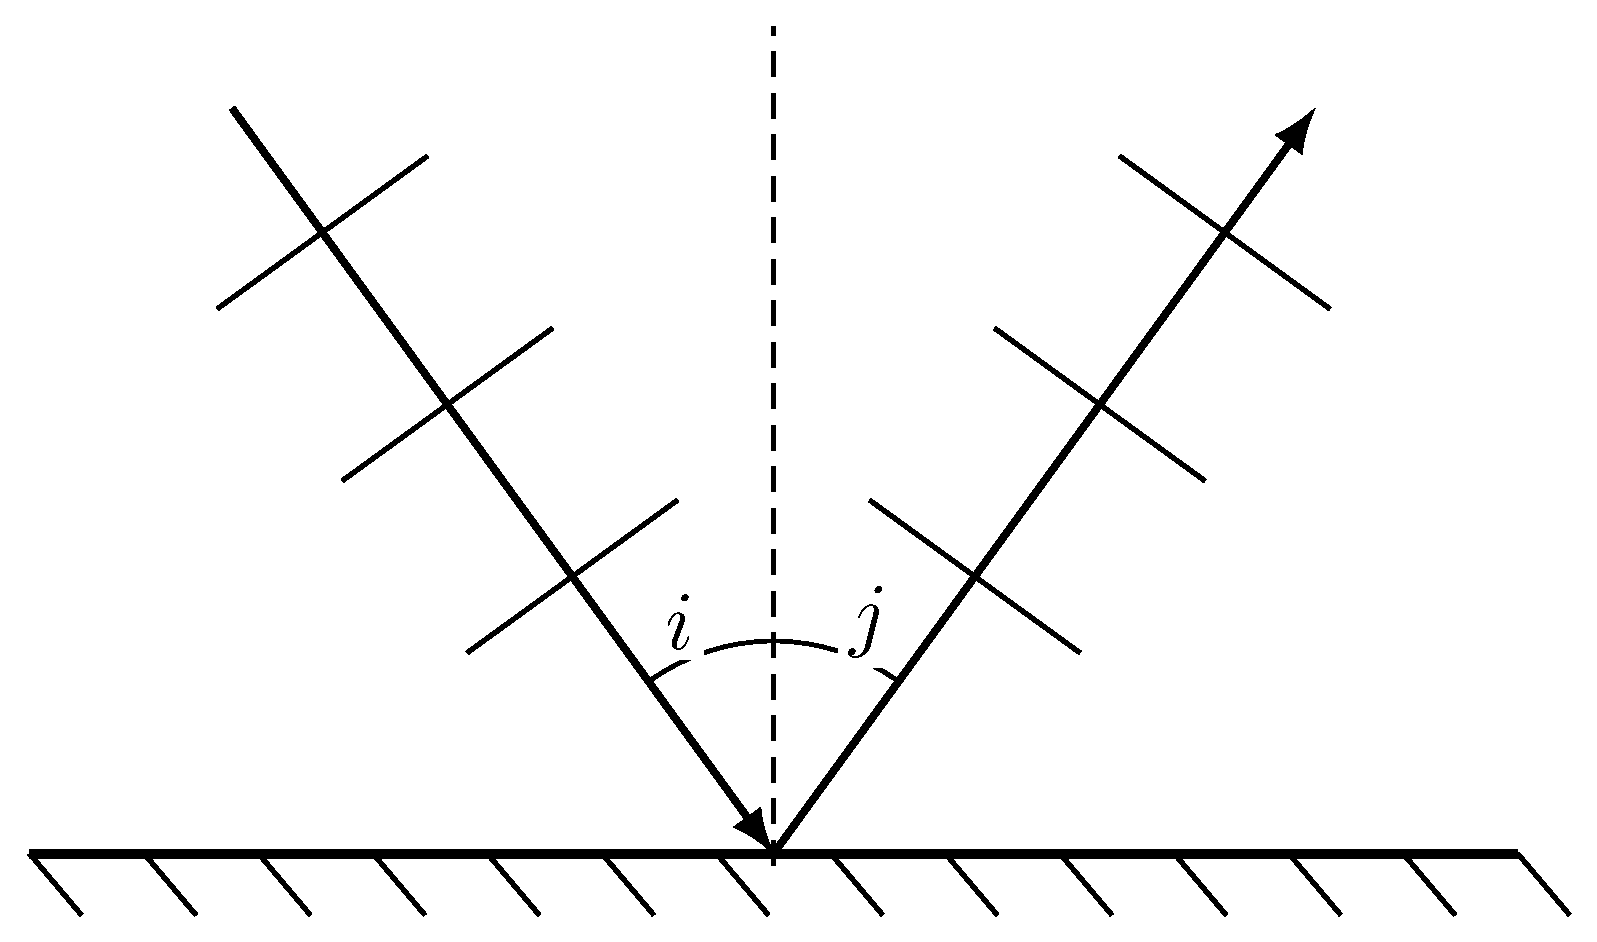
\includegraphics[keepaspectratio,width=58mm]{fig/n14_refl.png}
\end{zuright}

\bsNeed{44mm}
\begin{zuright}{58mm}
\hspace{1zw}次に{\gtfamily 屈折}を考える．水面波の速さは水深によって変わり，浅いところほど遅い．
右図のように，深いところ（速さ$v_1\U{m/s}$）から浅いところ（速さ$v_2\U{m/s}$）へ平面波が斜めに入射すると，境界に先に到達した側から順に波の進みが遅くなるため，波面の向きが変わる．
この現象を{\gtfamily 波の屈折}といい，法線と屈折波の進行方向のなす角を{\gtfamily 屈折角}$r$という．

\hspace{1zw}ここで重要なのは，{\gtfamily 境界を越えても波の振動数は変わらない}ことである．
波源が$1\U{s}$あたりに送り出した波の数は，境界で増えたり減ったりしないからである．
\zusep
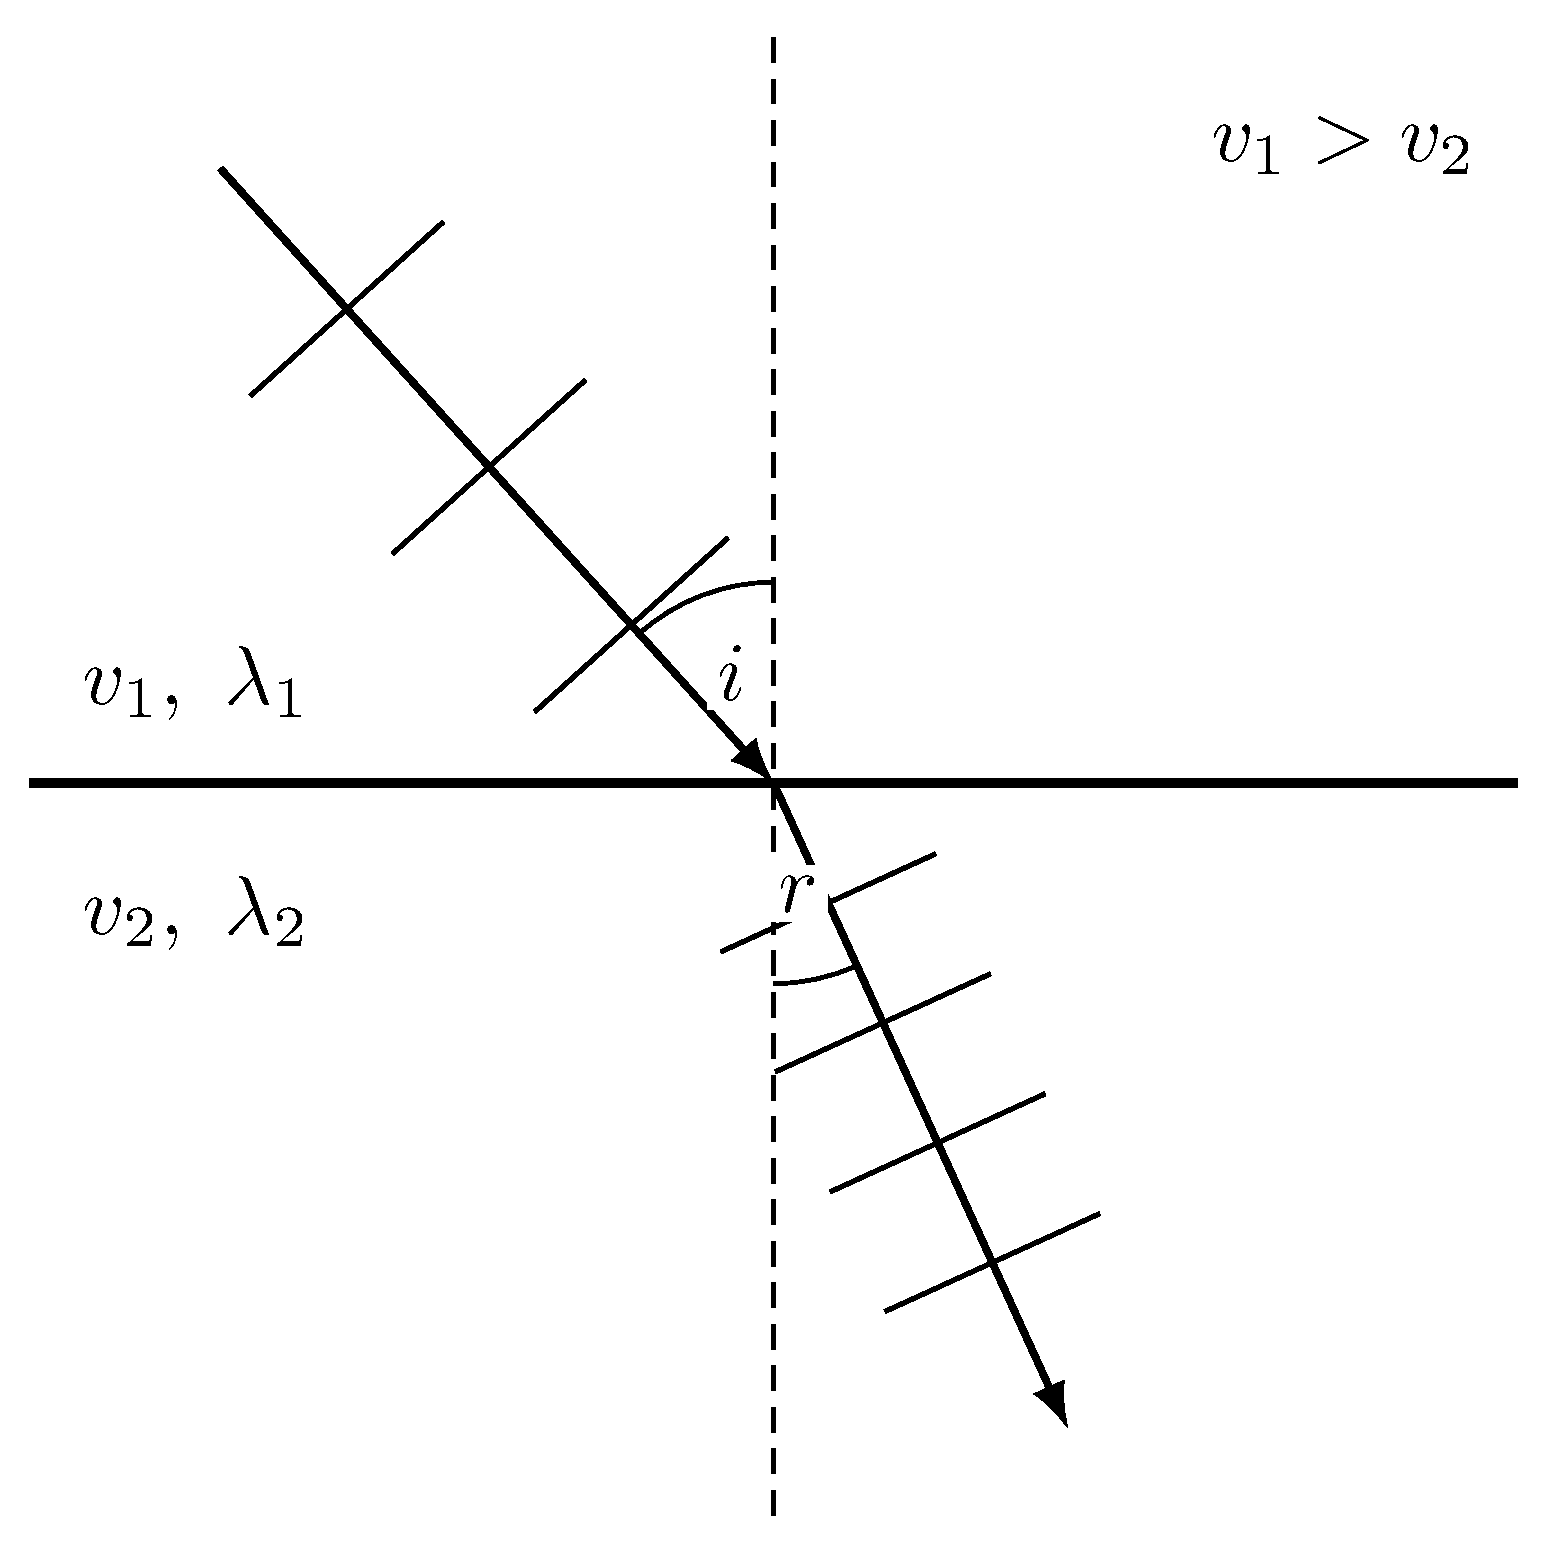
\includegraphics[keepaspectratio,width=58mm]{fig/n14_refr.png}
\end{zuright}

したがって$v=f\lambda$より，速さが変われば波長も同じ割合で変わることになる．
% 加筆（2026-09-14 ユーザー指摘）：λ1・λ2 は図（fig/n14_refr.png）にはラベルがあるが
%   本文では式の中が初出で，どちらが入射側か本文だけでは分からなかった。
入射側（速さ$v_1\U{m/s}$）の波長を$\lambda_1\U{m}$，屈折側（速さ$v_2\U{m/s}$）の波長を$\lambda_2\U{m}$とすると，振動数$f\U{Hz}$が共通であることから$v_1=f\lambda_1$, $v_2=f\lambda_2$，すなわち$\dfrac{v_1}{v_2}=\dfrac{\lambda_1}{\lambda_2}$である．
このとき，入射角$i$と屈折角$r$の間には
\[\dfrac{\sin i}{\sin r}=\dfrac{v_1}{v_2}=\dfrac{\lambda_1}{\lambda_2}\]
が成り立つ．これを{\gtfamily 屈折の法則}という（この式がホイヘンスの原理から導けることは，第18回 18.4 で光を例にとって示す）．

\begin{matome}{波の反射・屈折}
\hspace{3mm} 反射の法則\quad{}$\Rightarrow$\quad{}入射角 ＝ 反射角\\
\hspace{3mm} 屈折の法則\quad{}$\Rightarrow$\quad{}$\dfrac{\sin i}{\sin r}=\dfrac{v_1}{v_2}=\dfrac{\lambda_1}{\lambda_2}$\\
\hspace{3mm} 反射・屈折のいずれでも{\gtfamily 波の振動数は変化しない}（変わるのは速さと波長）
\end{matome}


\newpage

% 練習番号：波動は第2章の先頭なので［1］から始まる
\setcounter{qno}{0}

\filbreak
\Rank{A問題}

\Mon{基本事項の確認}

% 原本 第19回［1］に，原本 第20回［9］の(1)(2)（縦波の横波表示）を (5)(6) として加えた．
% ※ この回は 14.6 で縦波を扱うので，縦波の基本確認もここに置く（2026-09-04 ユーザー指示）。
%    第15回を組むときは，原本［9］は (3)(4)(5)（水面波の干渉・定常波・うなり）だけを
%    ㉑［16］と統合すること。(1)(2) はここへ移したので重複させない。
\begin{zuright}{60mm}
\hspace{1zw}以下の設問に答えよ．
\begin{komon}
\ko{1} 伝播速度$1.2\U{m/s}$，振動数$2.0\U{Hz}$の波の波長は何$\U{m}$か．
\ko{2} 波長$3.0\U{m}$，周期$2.0\U{s}$の波の伝播速度は何$\U{m/s}$か．
\ko{3} 正弦波を次のように観察したときにはそれぞれどのように見えるか．簡単に説明せよ．\\
       \hspace*{1zw}\MARU{1} 媒質の一点のみを観察する\\
       \hspace*{1zw}\MARU{2} 波の波形を観測する
\ko{4} 変位が$y(x,t)=0.3\sin\pi(t-0.5x)\U{m}$で表される波の振幅$A\U{m}$，周期$T\U{s}$，波長$\lambda\U{m}$を求めよ．
\ko{5} 右図は$x$軸方向に進行する縦波について，$+x$の向きの変位を$+y$の向きに取り直して横波表示したものである．媒質の右向きの変位が最大の点の$x$座標はいくらか．$0\leqq x<0.20\U{m}$の範囲で答えよ．
\ko{6} また，(5)の波動について，媒質の密度が最大の点および最小の点の$x$座標はいくらか．$0\leqq x<0.20\U{m}$の範囲で答えよ．
\end{komon}
\zusep
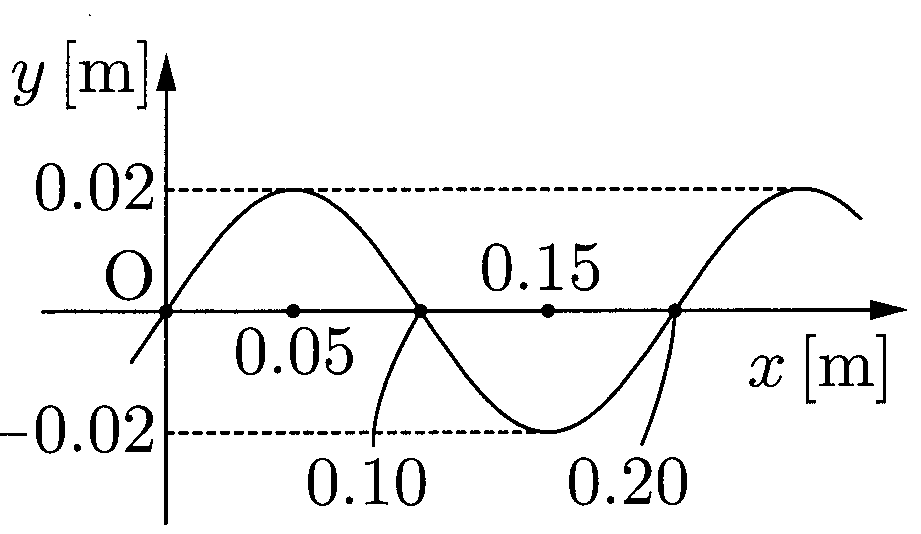
\includegraphics[keepaspectratio,width=60mm]{fig/n14_p1_long.png}
\end{zuright}

\filbreak
\Rank{B問題}

\Mon{横波と媒質の振動}

\begin{zuright}{60mm}
\hspace{1zw}右の図は，$x$軸の正の向きに伝わる正弦波の波形を示している．媒質が次の状態になっている位置は$\mathrm{A}\sim\mathrm{E}$のどこか．
\begin{komon}
\ko{1} 媒質の速さが0の位置．
\ko{2} 媒質の速度が上向き最大の位置．
\ko{3} 媒質の加速度が0の位置．
\ko{4} 媒質の加速度が上向き最大の位置．
\end{komon}
\zusep
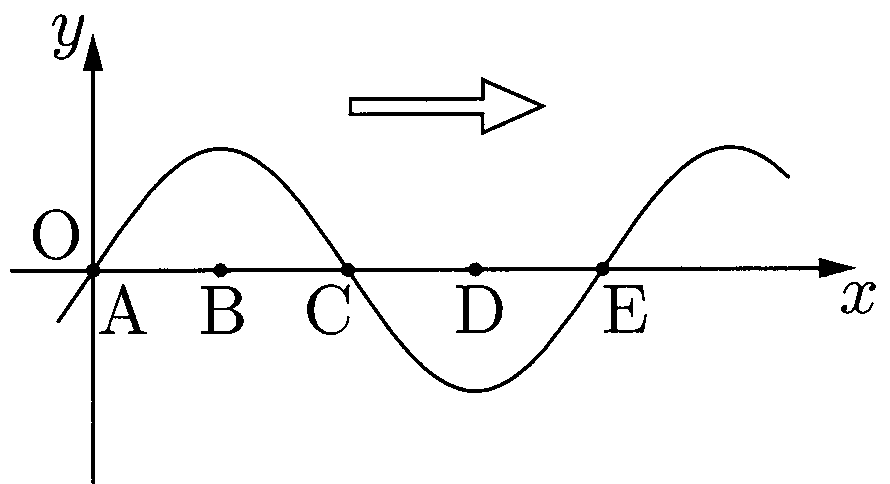
\includegraphics[keepaspectratio,width=60mm]{fig/n14_p2_wave.png}
\end{zuright}

\Mon{正弦波のグラフ}

\begin{zuright}{60mm}
\hspace{1zw}右図はある瞬間における正弦波の波形を示しており，この瞬間において，図中の媒質$\mathrm{A}$は下向き（矢印の方向）に動いている．これについて以下の設問に答えよ．
\begin{komon}
\ko{1} 波はどちら向きに進んでいるか．
\ko{2} この瞬間の媒質$\mathrm{B}$，$\mathrm{C}$の速度はどちら向きか．
\ko{3} この瞬間から1.5周期後の波形を点線で記入せよ．
\end{komon}
\zusep
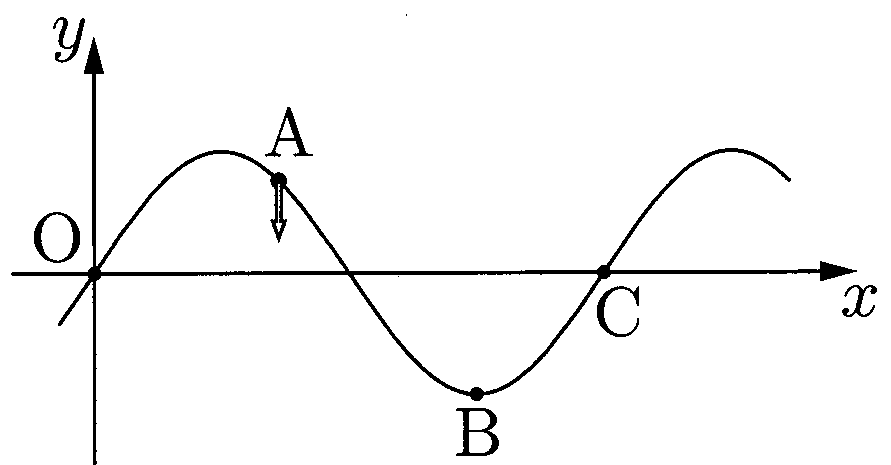
\includegraphics[keepaspectratio,width=60mm]{fig/n14_p3_wave.png}
\end{zuright}

\Mon[\Sitei]{$y-x$グラフ}

\begin{zuright}{54mm}
\hspace{1zw}右図のグラフは，周期$T\U{s}$，速さ$v\U{m/s}$，振幅$A\U{m}$で$x$軸の正の向きに進行している正弦波の，時刻$t=0\U{s}$における波形を示したものである．これについて以下の設問に答えよ．
\begin{komon}
\ko{1} この波の振動数$f\U{Hz}$と波長$\lambda\U{m}$を求めよ．
\ko{2} グラフの$x$, $y$座標の代表点に値を記入せよ．
\ko{3} (2)を元に，時刻$t=0\U{s}$における波の変位$y(x,0)$を表す方程式を求めよ．
\ko{4} 任意の時刻$t\U{s}$，位置$x\U{m}$における波の変位$y(x,t)$を表す方程式を求めよ．
\end{komon}
\zusep
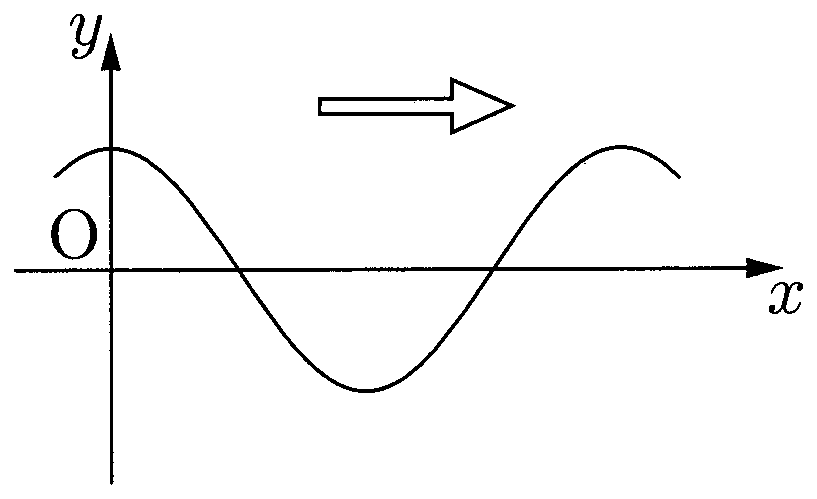
\includegraphics[keepaspectratio,width=54mm]{fig/n14_p4_yx.png}
\end{zuright}

\Mon[\Sitei]{$y-t$グラフ}

\begin{zuright}{58mm}
\hspace{1zw}右図のグラフは周期$T\U{s}$，速さ$v\U{m/s}$，振幅$A\U{m}$で$x$軸の\underline{負の向き}に進行している正弦波の，原点$x=0\U{m}$における振動を，横軸に時刻$t\U{s}$，縦軸に変位$y\U{m}$をとって表したものである．これについて以下の設問に答えよ．
\begin{komon}
\ko{1} グラフの$t$, $y$座標の代表点（$t$軸を切る時刻およびグラフの極大・極小値）に値を記入せよ．
\ko{2} 原点$x=0\U{m}$における波の変位$y(0,t)\U{m}$を表す式を求めよ．
\ko{3} 任意の時刻$t\U{s}$，位置$x\U{m}$における波の変位$y(x,t)\U{m}$を表す式を求めよ．
\end{komon}
\zusep
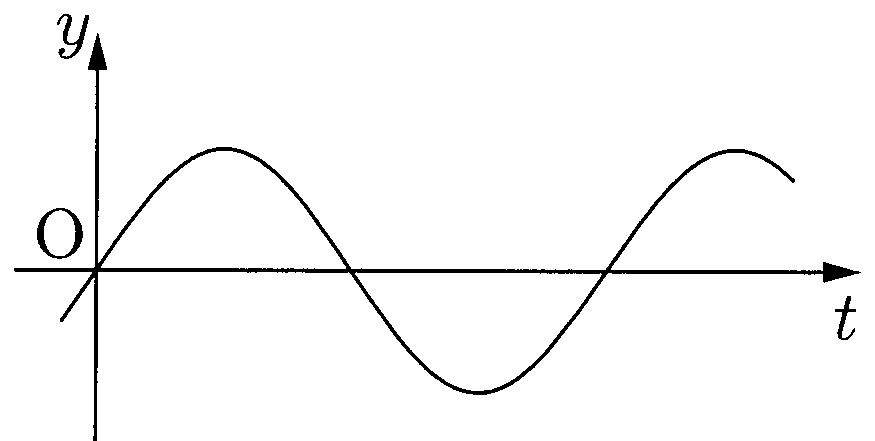
\includegraphics[keepaspectratio,width=58mm]{fig/n14_p5_yt.png}
\end{zuright}

\Mon{$y-x$グラフと$y-t$グラフの相互変換}

\begin{zuright}{58mm}
\hspace{1zw}右図のグラフは，周期$T\U{s}$，波長$\lambda\U{m}$，振幅$A\U{m}$で$x$軸正の向きに伝わる正弦波の，時刻$t=0\U{s}$における波形を，横軸に座標$x\U{m}$を，縦軸に変位$y\U{m}$をとって表したものである．これについて以下の設問に答えよ．
\begin{komon}
\ko{1} この正弦波が$+x$の向きに進行しているとして，原点$x=0\U{m}$における時刻$t\U{s}$の変位$y(0,t)\U{m}$を求めよ．
\ko{2} この正弦波が$-x$の向きに進行しているとして，原点$x=0\U{m}$における時刻$t\U{s}$の変位$y(0,t)\U{m}$を求めよ．
\ko{3} (2)について，まず与えられた$y-x$グラフを元に，任意の時刻$t\U{s}$，位置$x\U{m}$における波の変位$y(x,t)\U{m}$を表す方程式を求め，得られた方程式に$x=0\U{m}$を代入して(2)の答えに一致することを示せ．
\end{komon}
\zusep
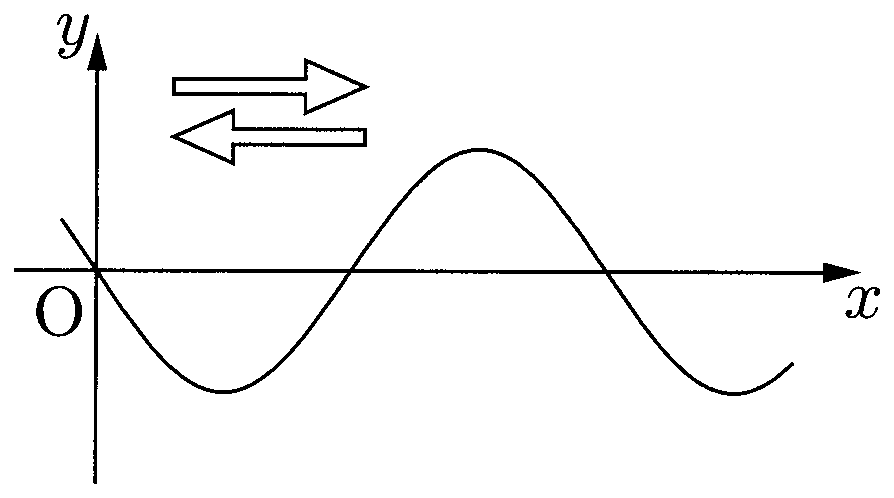
\includegraphics[keepaspectratio,width=58mm]{fig/n14_p6_conv.png}
\end{zuright}

% 再編：ここから 原本 第20回（20.1 縦波）の練習．講義の 14.6 縦波 に対応させて B問題の最後に置いた．
\Mon[\Sitei]{縦波の横波表示}

\begin{zuright}{70mm}
\hspace{1zw}右の図は，$x$軸の正の向きに伝わる縦波のある時刻における様子について，$+x$の向きの変位を$+y$の向きに取り直して横波表示したものである．以下の設問に答えよ．
\begin{komon}
\ko{1} もともと図の各点$\mathrm{A}\sim\mathrm{H}$にあった媒質は，このとき実際にはどの座標に変位しているか．それぞれ$\mathrm{A}^\prime\sim\mathrm{H}^\prime$として記入せよ．
\ko{2} 媒質の密度が最大の位置および最小の位置を点$\mathrm{A}\sim\mathrm{H}$から選べ．
\ko{3} 媒質の速さが$+x$の向きに最大となる位置，および$-x$の向きに最大となる位置を点$\mathrm{A}\sim\mathrm{H}$から選べ．
\end{komon}
\zusep
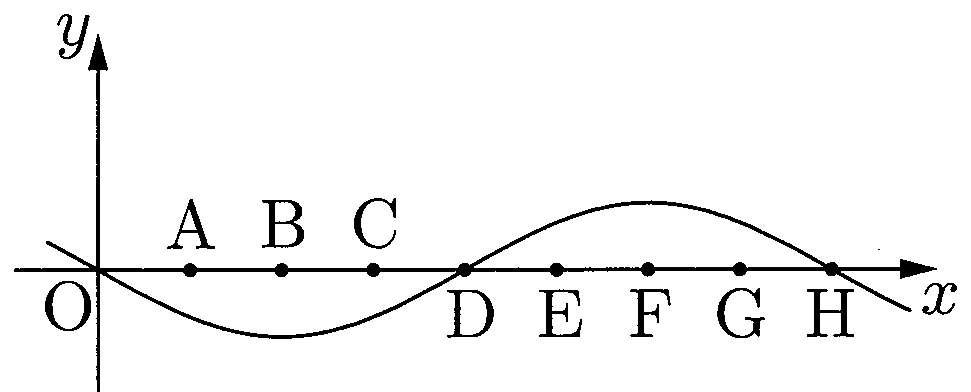
\includegraphics[keepaspectratio,width=70mm]{fig/n14_p7_long.png}
\end{zuright}

\filbreak
\Rank{C問題}

\Mon{波動の表式}

\hspace{1zw}$x$軸方向に伝わる正弦波があり，時刻$t\U{s}$における位置$x\U{m}$の振動の変位$y(x,t)\U{m}$が，$y(x,t)=a\sin(bt-cx)\U{m}$（ただし$a$, $b$, $c>0$）で与えられる．この波動について，以下の設問に答えよ．
\begin{komon}
\ko{1} この正弦波は$x$軸の正負どちらの向きに進行する波動か．
\ko{2} この波の振幅$A\U{m}$，波長$\lambda\U{m}$，周期$T\U{s}$，振動数$f\U{Hz}$，伝播速度$v\U{m/s}$を求めよ．
\end{komon}

\Mon{波の位相}

\begin{zuright}{66mm}
\hspace{1zw}$x$軸の正の向きに伝わる正弦波があり，右図は縦軸に媒質の変位$y\U{m}$，横軸に位置を表す座標$x\U{m}$をとり，ある時刻における変位を示したものである．以下の設問に答えよ．
\begin{komon}
\ko{1} 位置$\mathrm{A}$と位置$\mathrm{B}$における位相のずれの大きさ$\Delta\varphi\U{rad}$を求めよ．
\ko{2} 位置$\mathrm{A}$と同位相になっている位置を$\mathrm{B}$から$\mathrm{G}$の中から選べ．
\ko{3} 位置$\mathrm{A}$と逆位相になっている位置を$\mathrm{B}$から$\mathrm{G}$の中から選べ．
\end{komon}
\zusep
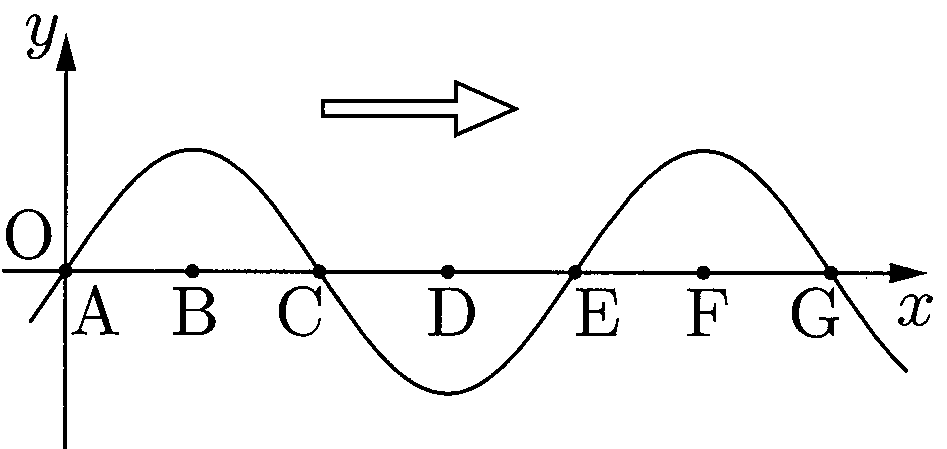
\includegraphics[keepaspectratio,width=66mm]{fig/n14_p9_phase.png}
\end{zuright}

\Mon{縦波と媒質の関係}

\begin{zuright}{54mm}
\hspace{1zw}$x$軸平行方向に伝わる縦波があり，右の二つのグラフは，媒質の$+x$の向きの変位を$+y$の向きの変位に取り直して横波表示にして図示したものである．図1は時刻$t=0\U{s}$の瞬間における媒質の変位と座標との関係を表す波形グラフであり，図2は原点$x=0\U{m}$の位置の変位が時刻$t$に対してどのように変化するのかを表したグラフである．この二つのグラフを参考にして，以下の設問に答えよ．
\begin{komon}
\ko{1} この縦波の進行の向きおよびその速さを求めよ．
\ko{2} $x=\dfrac{\lambda}{8}\U{m}$の点が密になる時刻を$0\leqq t<T\U{s}$の範囲で求めよ．
\ko{3} $t=\dfrac{3}{4}T\U{s}$のときに密度が密になる点を$0\leqq x<\lambda\U{m}$の範囲で求めよ．
\end{komon}
\zusep
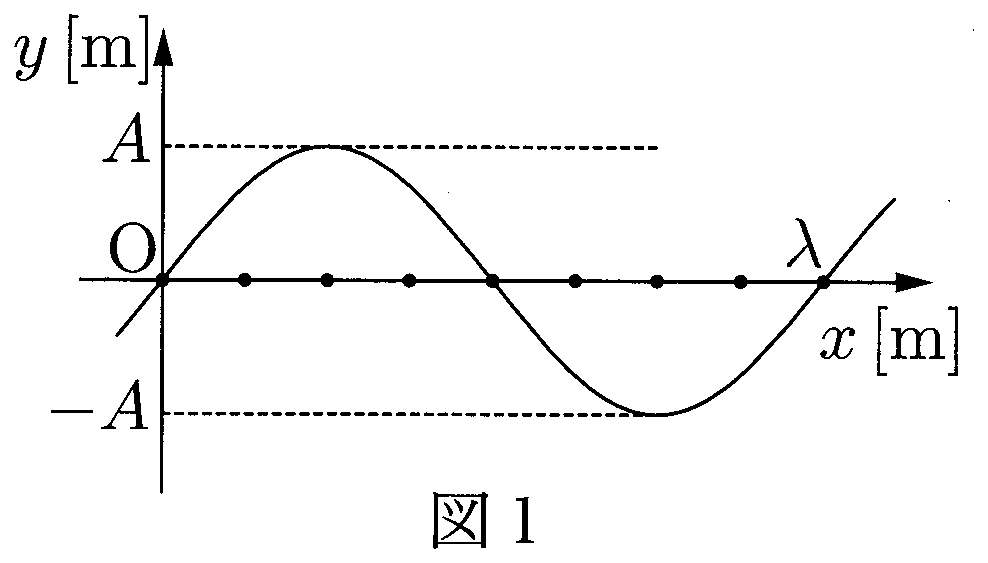
\includegraphics[keepaspectratio,width=54mm]{fig/n14_p10_fig1.png}\\[3mm]
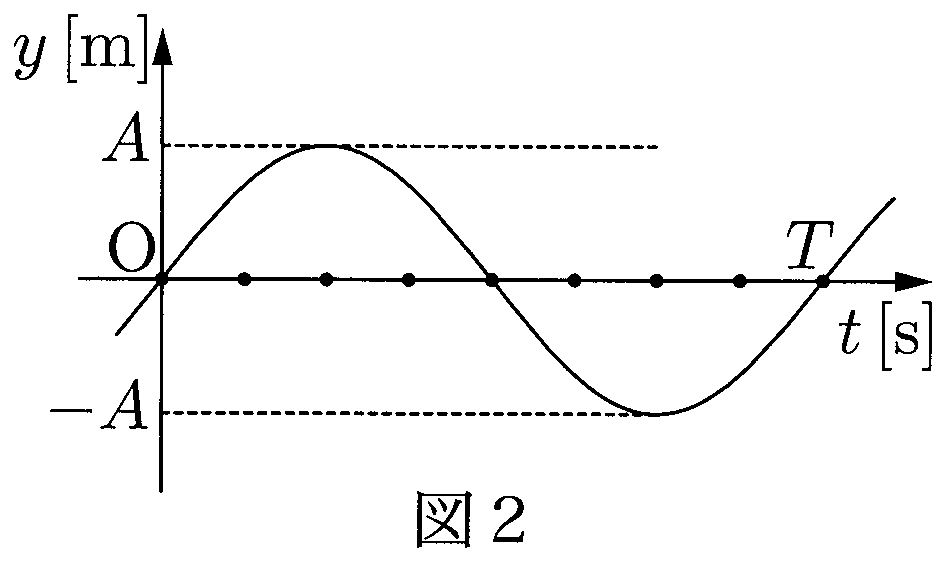
\includegraphics[keepaspectratio,width=54mm]{fig/n14_p10_fig2.png}
\end{zuright}


\newpage

\KaiTitle{第14回　正弦波の表式と縦波}
\setlength{\columnseprule}{0.4pt}
\begin{multicols}{2}
\raggedcolumns

\Rank{A問題}
\MonN{1}{基本事項の確認}\par\nopagebreak
\begin{sisin}
関係式$v=f\lambda$, $f=\dfrac{1}{T}$の利用，および正弦波についての考え方を整理せよ．(4)については，振幅・周期・波長が意味するところを考えれば求められる．

(5)(6)は横波表示した縦波の読み取り方．疎密判定はすぐに行えるように練習を繰り返すこと．
\end{sisin}
\KaiHead
\begin{komon}
\ko{1} $v=f\lambda$より，$\lambda=\dfrac{v}{f}=\dfrac{1.2}{2.0}=0.60\U{m}$\hspace*{\fill}\Ans
\ko{2} $f=\dfrac{1}{T}$より$v=f\lambda=\dfrac{1}{T}\cdot\lambda$であるから，
       \[v=\frac{\lambda}{T}=\frac{3.0}{2.0}=1.5\U{m/s}\Ans\]
\ko{3} \MARU{1} 媒質は波の進行の向きに対して垂直に単振動している．\hspace*{\fill}\Ans\\
       \MARU{2} 波の波形は，形をそのままに保ちながら波の進行の向きへとずれていく．\hspace*{\fill}\Ans
\ko{4} ある座標（例えば$x=0$）に着目する（すなわち$y(0,t)=0.3\sin\pi t$について考える）と，時刻$t$の変化により変位は$+0.3\sim-0.3\U{m}$の範囲で振動する．よって，$A=0.3\U{m}$\Ans．

       また，ある座標（例えば$x=0$）に着目すると，時刻$t$がちょうど$2.0\U{s}$だけずれると位相（三角関数の中味）が$2\pi$だけずれて元の変位に戻るので，波の周期は$T=2.0\U{s}$\Ans．

       また，ある時刻（例えば$t=0$）に着目する（すなわち$y(x,0)=0.3\sin(-0.5\pi x)\U{m}$について考える）と，座標$x$がちょうど$4.0\U{m}$だけずれると位相（三角関数の中味）が$2\pi$だけずれて元の変位に戻る（三角関数の中味の繰り返しが$4.0\U{m}$ごとに起こる）ので，波の波長は$\lambda=4.0\U{m}$．\hspace*{\fill}\Ans
\ko{5} 横波表示の$+y$の向きの変位が，実際の$+x$（右）の向きの変位である．よって$y$が最大となる山の位置を読み取って，
       \[x=0.05\U{m}\Ans\]
\ko{6} $x$が増加するにつれて変位が正から負へ変わる点では媒質が左右から集まるので密，負から正へ変わる点では媒質が左右へ遠ざかるので疎である．よって，
       \[\text{密度最大：}x=0.10\U{m}\]
       \[\text{密度最小：}x=0.00\U{m}\Ans\]
\end{komon}

\Rank{B問題}
\MonN{2}{横波と媒質の振動}\par\nopagebreak
\begin{sisin}
正弦波では，各質点は$y$軸の向きに単振動をしているだけで，質点そのものが$x$軸の向きに動いていくのではない．次の瞬間に各質点がどのように動くのかについては，次の瞬間の波形を作図し，媒質各点の上下方向への動きを把握すればよい．

また媒質の加速度については上述したような作図では分からない．単振動では，速さが0, 最大となるのは，それぞれ振動端点，中心点．また，加速度の大きさが0, 最大となるのは，それぞれ中心点，端点である．このことを用いて(3)・(4)を考えよ．
\end{sisin}
\KaiHead
\hspace{1zw}まず，図の$\mathrm{A}\sim\mathrm{E}$は$x$軸上にとってあるが，これは{\gtfamily 媒質の振動中心（もとの位置）の$x$座標}を示しているのであって，その媒質の\emph{いま}の変位は真上・真下にある波形上の点で読む．たとえば$\mathrm{B}$の媒質はいま山の頂点まで持ち上がっており，$\mathrm{D}$の媒質は谷の底まで下がっている．

\hspace{1zw}媒質各点は$y$軸方向に振幅，周期の等しい単振動をしている．この正弦波は右へ進んでいるので，次の瞬間の，ほんの少し右へずれた波形を描いてみると次図の破線のようになる．
\begin{center}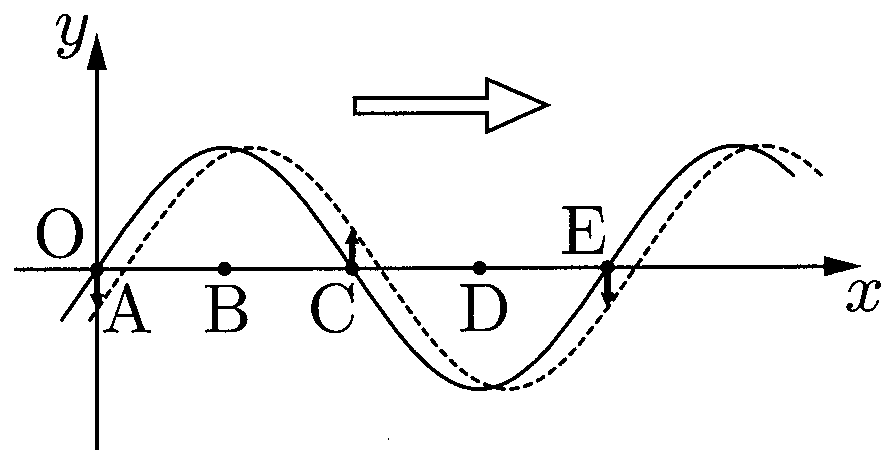
\includegraphics[keepaspectratio,width=62mm]{fig/n14_a2_wave.png}\end{center}
\hspace{1zw}すなわち，$\mathrm{A}$, $\mathrm{B}$, $\mathrm{C}$, $\mathrm{D}$, $\mathrm{E}$の媒質各点は，上図に示した$\Rightarrow$の向きへと次の瞬間に移動することが分かる．すなわち，
\[\mathrm{A}:\downarrow,\ \ \mathrm{B}:0,\ \ \mathrm{C}:\uparrow,\ \ \mathrm{D}:0,\ \ \mathrm{E}:\downarrow\]
へと移動する．
\begin{komon}
\ko{1} 媒質の速さが0となるのは，媒質が単振動の端点にいる，$\mathrm{B}$と$\mathrm{D}$\hspace*{\fill}\Ans
\ko{2} 媒質の速さが最大となるのは，単振動の中心を通過する$\mathrm{A}$, $\mathrm{C}$, $\mathrm{E}$であり，このうち媒質の速度が上を向いているのは，$\mathrm{C}$\hspace*{\fill}\Ans
\ko{3} 媒質の加速度が0となるのは媒質が単振動の振動中心を通過する瞬間であるから，$\mathrm{A}$, $\mathrm{C}$, $\mathrm{E}$\hspace*{\fill}\Ans
\ko{4} 媒質の加速度の大きさが最大となるのは，単振動の端点に媒質が来た瞬間である$\mathrm{B}$と$\mathrm{D}$である．単振動の加速度の向きと変位の向きとは逆向きであることから，$\mathrm{B}$, $\mathrm{D}$のうち，媒質の加速度が上を向いているのは，変位が負である$\mathrm{D}$\hspace*{\fill}\Ans
\end{komon}

\MonN{3}{正弦波のグラフ}\par\nopagebreak
\begin{sisin}
$\mathrm{A}$点が次の瞬間に下に動くためには，波形が右へずれればよいのか，それとも左へずれればよいのかを考えよ．これを考えれば波の進行の向きが分かる．

波の周期とは，\MARU{1}各点の媒質の上下単振動の周期，であると同時に，\MARU{2}正弦波の波形が進行の向きに1波長分だけずれるのに要する時間，でもある．\MARU{2}の考え方を使えば分かりやすい．
\end{sisin}
\KaiHead
\begin{komon}
\ko{1} 波が右に動いている場合，および左に動いている場合について，それぞれ次の瞬間の波形を図示すると次図のようになる．
       \begin{center}
       ・右へ進む場合\\[1mm]
       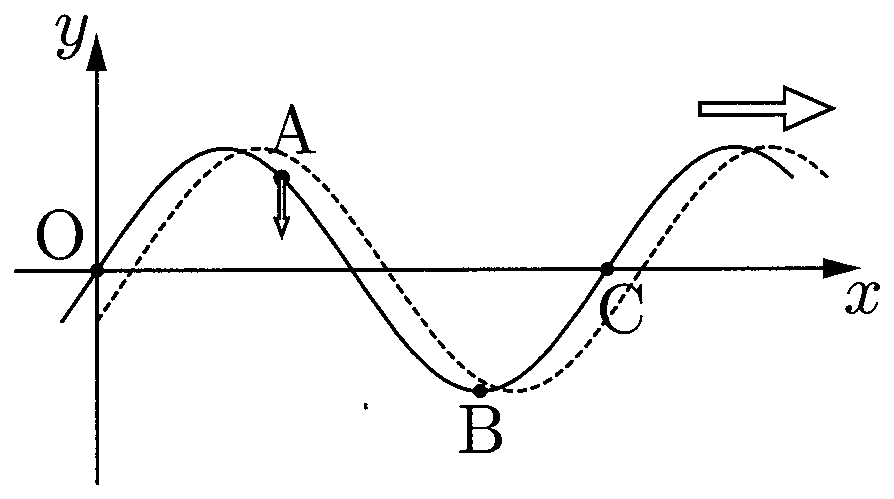
\includegraphics[keepaspectratio,width=62mm]{fig/n14_a3_right.png}\\[2mm]
       ・左へ進む場合\\[1mm]
       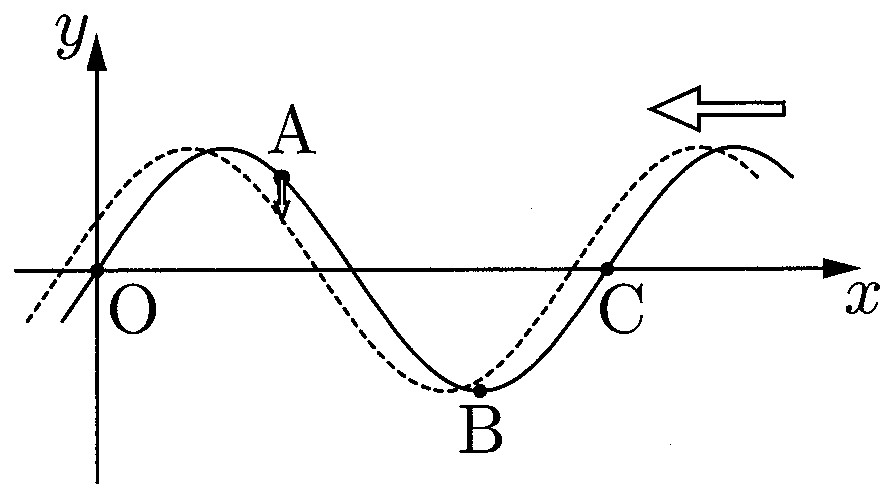
\includegraphics[keepaspectratio,width=62mm]{fig/n14_a3_left.png}
       \end{center}
       上図から分かるように，$\mathrm{A}$点が次の瞬間に下へ移動するのは，波動が左へ進行している場合である．よって，波は左へと進行している．\hspace*{\fill}\Ans
\ko{2} 上の図から$\mathrm{B}$, $\mathrm{C}$点の移動する向きを読み取ると，
       \[\mathrm{B}\text{点：速度}0\text{（向きなし）}\]
       \[\mathrm{C}\text{点：速度は上向き}\Ans\]
\end{komon}
\begin{chuu}
上図を見ると，$\mathrm{B}$点は次の瞬間，上向きに動いているように見えるが，これは考えている「次の瞬間」が，実際には微小時間後ではないためである．左へずらす距離をもっと小さくしていくと，$\mathrm{A}$や$\mathrm{C}$点の動きの大きさに比べて，$\mathrm{B}$点の動きはほぼ0になる．

単振動の端点に来ている$\mathrm{B}$点であれば媒質の移動速度は0である，ということは覚えておき，作図に惑わされないようにせよ．
\end{chuu}
\begin{komon}
\ko{3} 1周期たつと，波形はその進行の向きに1波長分だけずれるので，1.5周期だけ時間がたつと，波形は進行の向きに1.5波長分だけずれる．よって，波形を左の向きに1.5波長分だけずらした図を作図すると，次図の点線のようなグラフが得られる．
       \begin{center}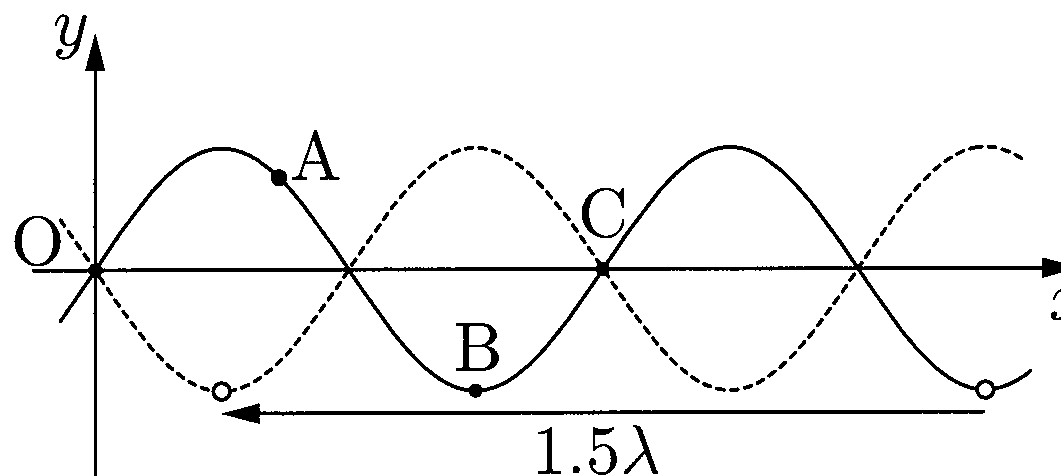
\includegraphics[keepaspectratio,width=62mm]{fig/n14_a3_15T.png}\end{center}
       （図中の白$\bigcirc$の点と同様に，波形全体が左の向きへと1.5波長分だけずれている）
\end{komon}
\begin{bekkai}
波形の繰り返し単位の長さが1波長なのであるから，波形は右もしくは左の向きに整数波長分だけずれても見かけ上は全く同一の波の形になる．よって，1.5波長分だけ波がずれたときの波形は，0.5波長分だけ波がずれたときと同じ波形になる．

また，0.5波長分，すなわち半波長分だけ波がずれた場合は，波形はちょうど$x$軸に対して折り返した正負逆の波形になる．以上より，1.5周期後の波形とは，与えられた波形グラフを正負反転させた波形になるので，次図を得る．
\begin{center}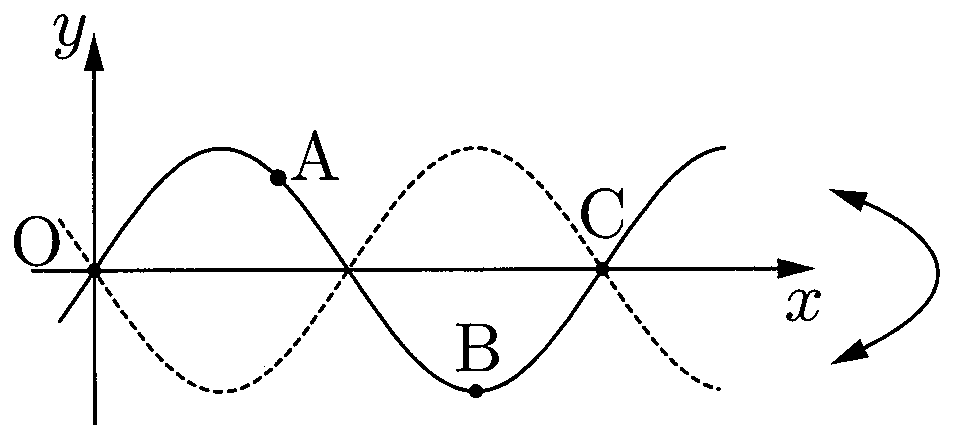
\includegraphics[keepaspectratio,width=62mm]{fig/n14_a3_bekkai.png}\end{center}
\end{bekkai}

\MonN{4}{$y-x$グラフ}\par\nopagebreak
\begin{sisin}
関係式$v=f\lambda$, $f=\dfrac{1}{T}$はしっかりと覚えておくこと．代表点の値は，波長や振幅の意味するところを考えれば記入できるはずである．与えられているグラフが$t=0\U{s}$の瞬間における{\gtfamily 波形のグラフ}であることに注意して考えよう．

$t=0\U{s}$の$y-x$グラフを元に一般表式$y(x,t)$を得るためには，時刻$t\U{s}$における位置$x\U{m}$の振動が{\gtfamily 時刻$t=0\U{s}$には} どの地点にあった振動であるかを考えればよい．式を暗記して利用するのではなく，そのつどこのことを考えれば間違いがない．
\end{sisin}
\KaiHead
\begin{komon}
\ko{1} 振動数，周期，波速，波長の間に成り立つ関係より，
       \[f=\frac{1}{T}\U{Hz},\hspace{4mm}\lambda=\frac{v}{f}=vT\U{m}\Ans\]
\ko{2} 振幅は波形の振れ幅であり，また波長とは波形の繰り返し単位の長さであることから，以下のように代表点を記入できる．
       \begin{center}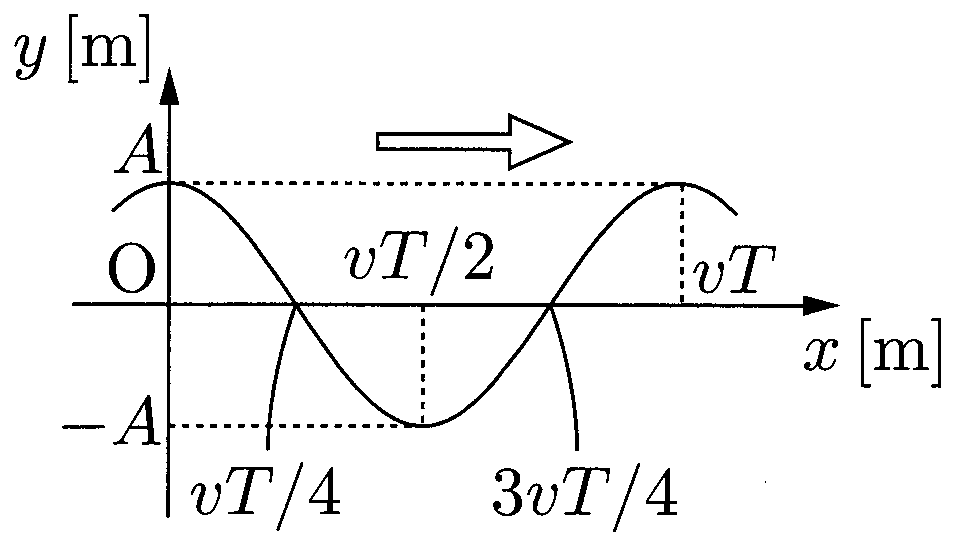
\includegraphics[keepaspectratio,width=62mm]{fig/n14_a4_daihyo.png}\end{center}
       \hspace*{\fill}\Ans
\ko{3} (2)のグラフを数式化すると，
       \[y(x,0)=A\cos\left(2\pi\frac{x}{vT}\right)\U{m}\Ans\]
\end{komon}
\begin{chuu}
(2)のグラフから(3)の答えの数式がパッと導けない人も多いだろう．そのような人は，まず(3)の答えの数式をグラフ化したら(2)の答えになることをチェックして欲しい．これが理解できれば(2)のグラフから(3)の数式を導くのは簡単である．まず，与えられたグラフは$x=0\U{m}$で最大値$A\U{m}$をとる山から始まっているから，
% 原本は「三角関数のカーブの形はこれは…」と文がねじれている（推敲漏れ）ので整えた．
$y(x,0)=+A\cos(\cdots\cdots)$という形の数式になることが分かる．三角関数の中味の部分（位相）については，$x$座標の繰り返し単位（波長）が$vT\U{m}$であることから，三角関数の中味の部分は，$x$座標が$vT\U{m}$だけずれると$2\pi\U{rad}$だけずれて元と同じ値になるような式であると考えられる．よって三角関数の中味は$2\pi\times\dfrac{x}{vT}$であり，これを先の三角関数の概形の式$y(x,0)=+A\cos(\cdots\cdots)$に入れれば(3)が得られる．
\end{chuu}
\begin{komon}
\ko{4} 時刻$t\U{s}$，位置$x\U{m}$での変位は，時刻$t=0\U{s}$においては$x-vt\U{m}$の位置での変位に等しいはずである．
       \begin{center}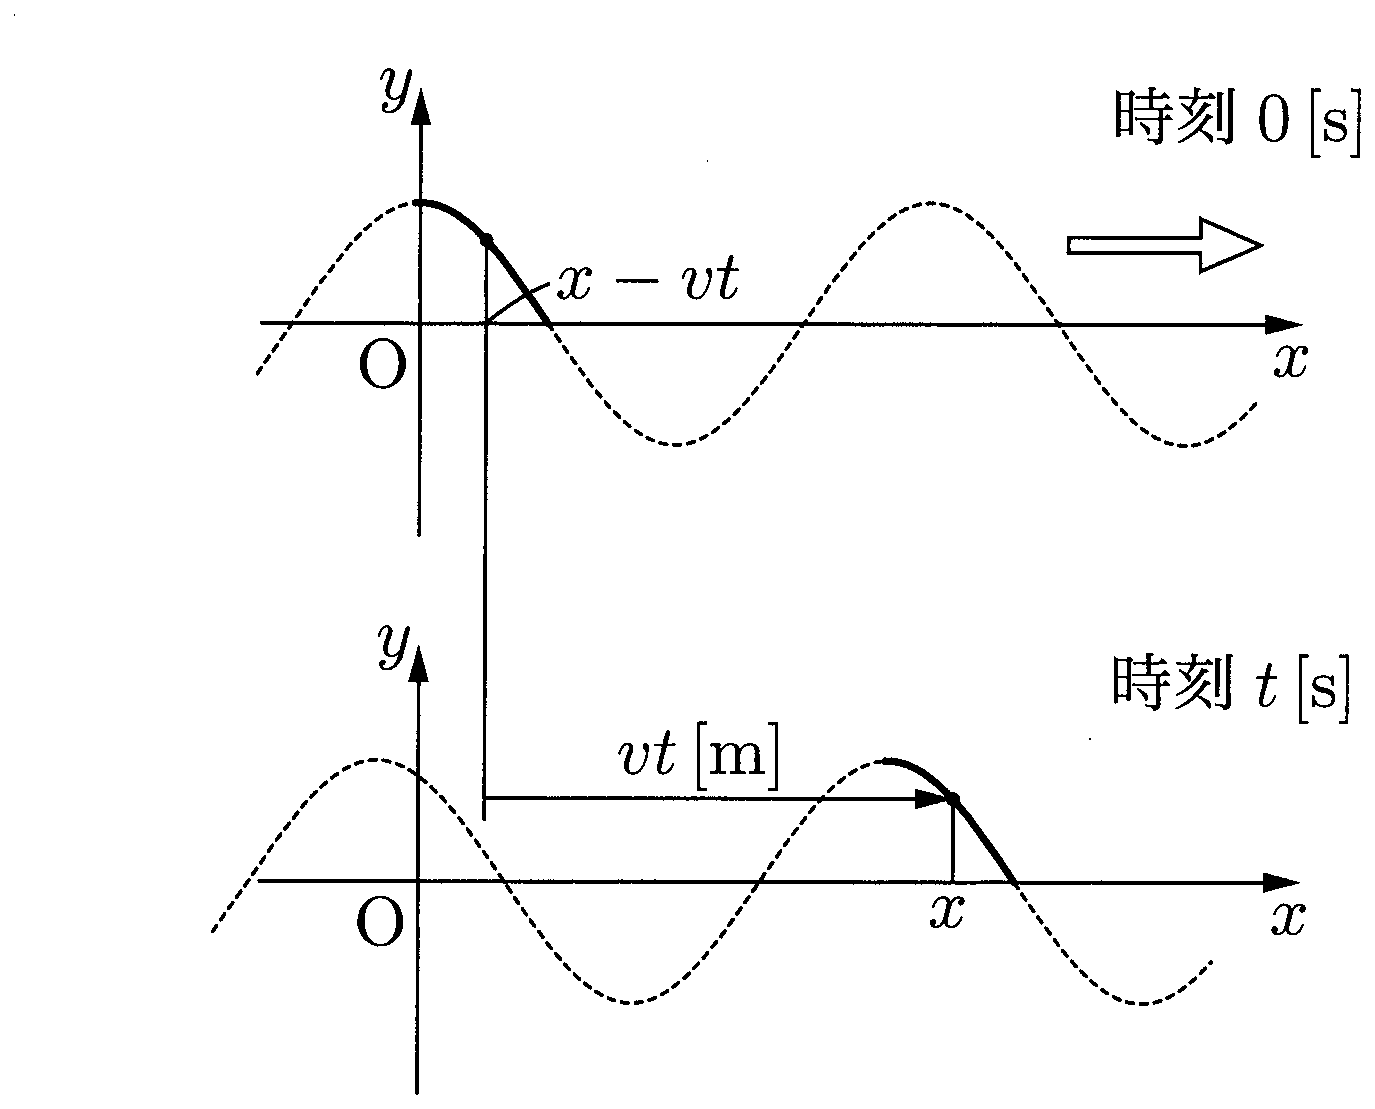
\includegraphics[keepaspectratio,width=62mm]{fig/n14_a4_shift.png}\end{center}
       よって，
       \[y(x,t)=y(x-vt,0)=A\cos\left(2\pi\frac{x-vt}{vT}\right)\]
       \[=A\cos 2\pi\left(\frac{x}{vT}-\frac{t}{T}\right)\U{m}\Ans\]
\end{komon}

\MonN{5}{$y-t$グラフ}\par\nopagebreak
\begin{sisin}
前問と違い，$y-t$グラフが与えられている．グラフの形は前問と似てはいるが，このグラフは{\gtfamily 波形を表してはいない}．

任意の時刻における$x=0\U{m}$の変位が与えられている．一般表式$y(x,t)$を得るためには，既知である$x=0\U{m}$の変位に直して考えればよい．すなわち，時刻$t\U{s}$における位置$x\U{m}$の振動が，$x=0\U{m}$をいつ通過するのかを考えればよい．
\end{sisin}
\KaiHead
\begin{komon}
\ko{1} 原点の単振動の周期は，波動の周期$T\U{s}$に一致すること，また単振動の振幅は波動の振幅$A\U{m}$に一致することに注意すると，代表点は次図のように記入できる．
       \begin{center}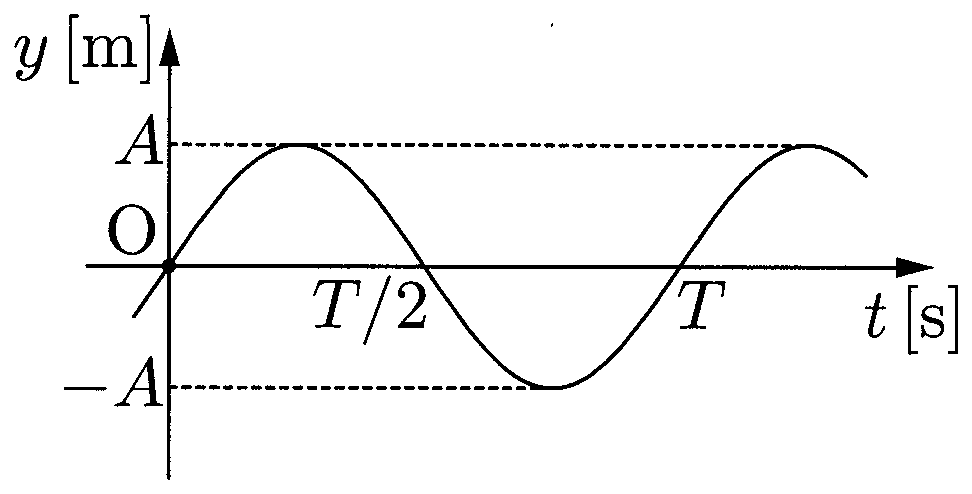
\includegraphics[keepaspectratio,width=62mm]{fig/n14_a5_daihyo.png}\end{center}
       \hspace*{\fill}\Ans
\ko{2} (1)のグラフを数式化すると，
       \[y(0,t)=A\sin\left(2\pi\frac{t}{T}\right)\U{m}\Ans\]
\end{komon}
\begin{chuu}
(1)のグラフの数式化も前問と全く同様なやり方で行えばよい．
\end{chuu}
\begin{komon}
\ko{3} この波は速さ$v\U{m/s}$で$x$軸負の向きに進行していることに注意すると，時刻$t\U{s}$に位置$x\U{m}$に存在する波は，時間$\dfrac{x}{v}\U{s}$を要して原点に達するので，この波が原点を通過するのは時刻$t+\dfrac{x}{v}\U{s}$になる．
       \begin{center}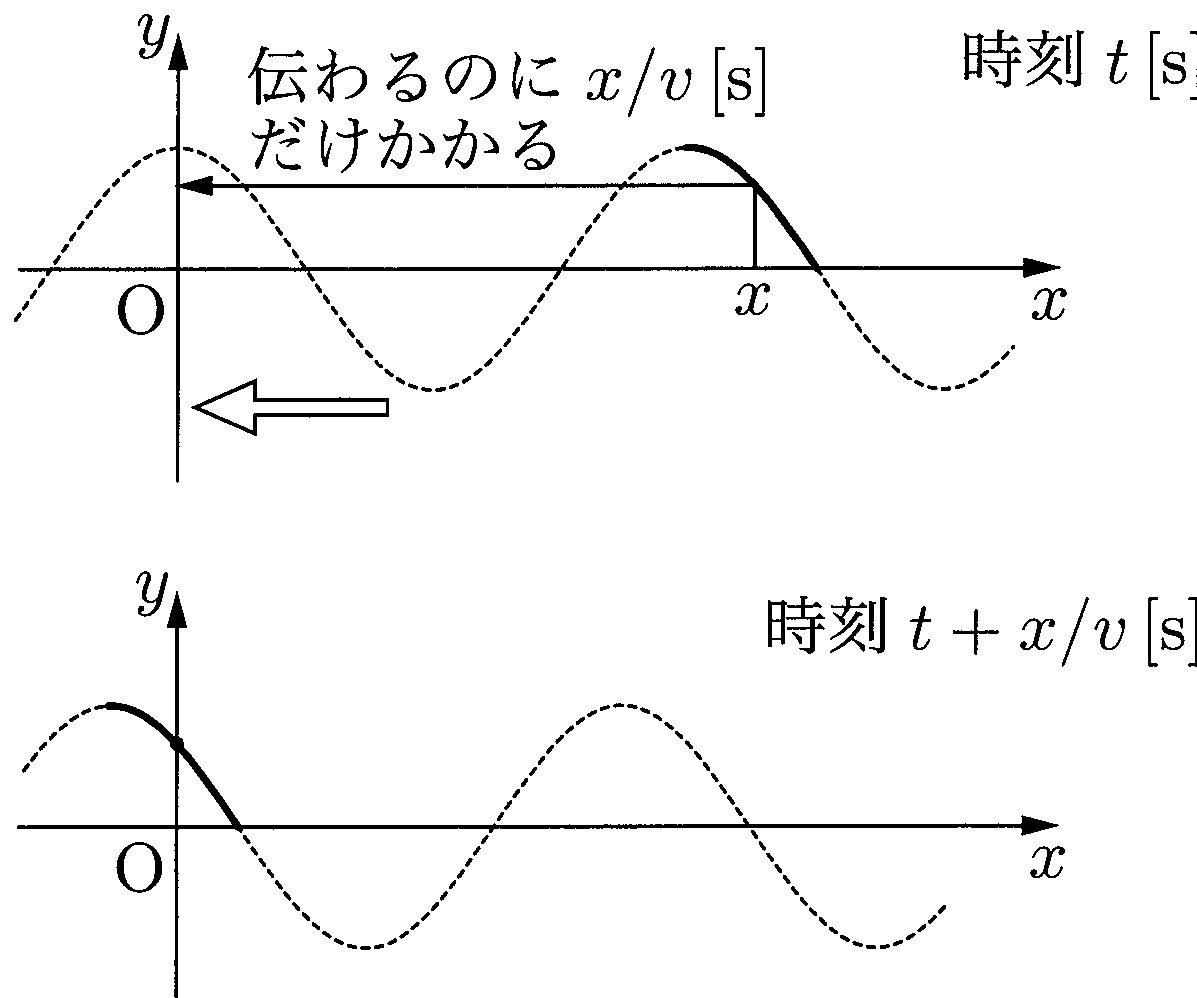
\includegraphics[keepaspectratio,width=62mm]{fig/n14_a5_shift.png}\end{center}
       よって，
       \[y(x,t)=y\left(0,\,t+\frac{x}{v}\right)=A\sin\left(2\pi\frac{t+x/v}{T}\right)\]
       \[=A\sin 2\pi\left(\frac{t}{T}+\frac{x}{vT}\right)\U{m}\Ans\]
\end{komon}
\begin{chuu}
問題文で与えられているグラフが$y-t$グラフであっても，$y(x,t)$の表式を得るために考えるのは時刻$t\U{s}$における$y-x$グラフ（波形グラフ）である．$y-x$グラフが与えられている場合も，$y-t$グラフが与えられている場合も，考えなければならないのは，時刻$t\U{s}$, 位置$x\U{m}$における波の変位$y(x,t)$が，与えられた既知のグラフのどの点に対応しているのかである．それを考えるためには，波形グラフを持ちだし，これがどのように時間的に移動しているのかを考えなければならない．
\end{chuu}

\MonN{6}{$y-x$グラフと$y-t$グラフの相互変換}\par\nopagebreak
\begin{sisin}
原点にある媒質の上下の単振動は，振幅が$A\U{m}$，周期が$T\U{s}$の単振動になることは明らかであるが，この条件を満たす単振動の式は，例えば$y(0,t)=A\sin 2\pi\dfrac{t}{T}$, $-A\sin 2\pi\dfrac{t}{T}$, $A\cos 2\pi\dfrac{t}{T}$, $-A\cos 2\pi\dfrac{t}{T}$などさまざまなものが考えられるが，これらのいずれに相当するのかは，時刻$t=0\U{s}$の媒質の変位，およびその次の瞬間に媒質の動く向きによって見分けることができる．そこで，与えられた波形グラフを少し進めてみて，原点の媒質がどちらの向きに動き出すのかを判定する．それが分かったら，あとは振幅が$A\U{m}$，周期が$T\U{s}$の単振動となるような$y-t$グラフを作図し，これをグラフ化すればよい．
\end{sisin}
\KaiHead
\hspace{1zw}媒質各点の上下振動は振幅$A\U{m}$，周期$T\U{s}$の単振動である．また，時刻$t=0\U{s}$における原点$x=0\U{m}$の変位は$y=0\U{m}$である．
\begin{komon}
\ko{1} 正弦波は$x$軸正の向きに進行しているので，次の瞬間の波形を描くと次の図の破線のようになる．
       \begin{center}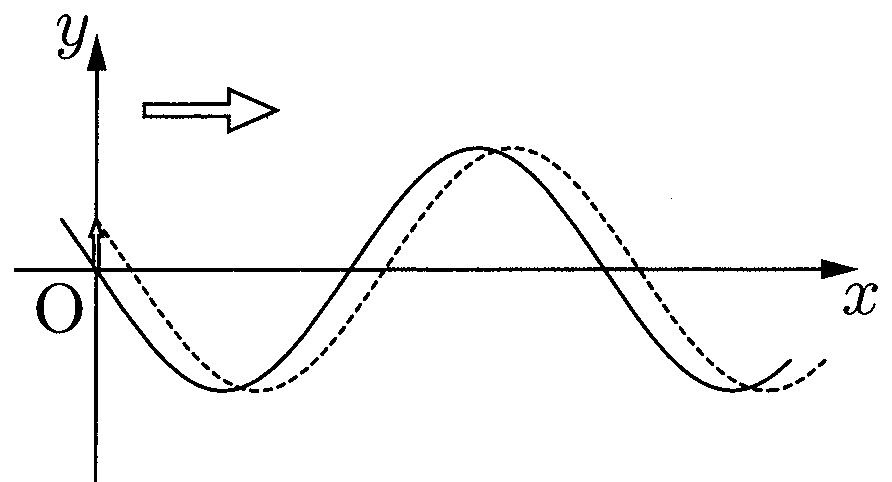
\includegraphics[keepaspectratio,width=62mm]{fig/n14_a6_1a.png}\end{center}
       よって，次の瞬間，原点の媒質は$+y$の向きに動き出すと分かる．振幅$A\U{m}$，周期$T\U{s}$，時刻$t=0\U{s}$における変位が$y=0\U{m}$で$+y$の向きに動き出す単振動という条件を満たす単振動の時間変動のグラフは次の$y-t$グラフのようなものに限られる．
       \begin{center}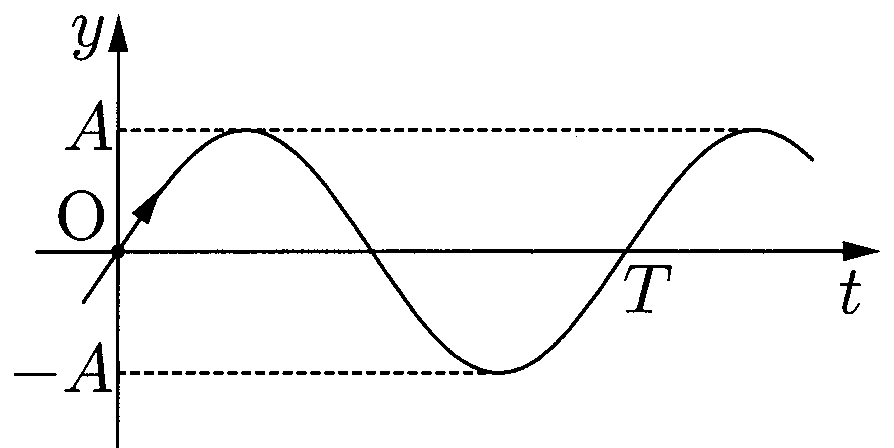
\includegraphics[keepaspectratio,width=62mm]{fig/n14_a6_1b.png}\end{center}
       これを数式化すると，
       \[y(0,t)=A\sin 2\pi\frac{t}{T}\U{m}\Ans\]
\ko{2} 正弦波は$x$軸負の向きに進行しているので，次の瞬間の波形を描くと次の図の破線のようになる．
       \begin{center}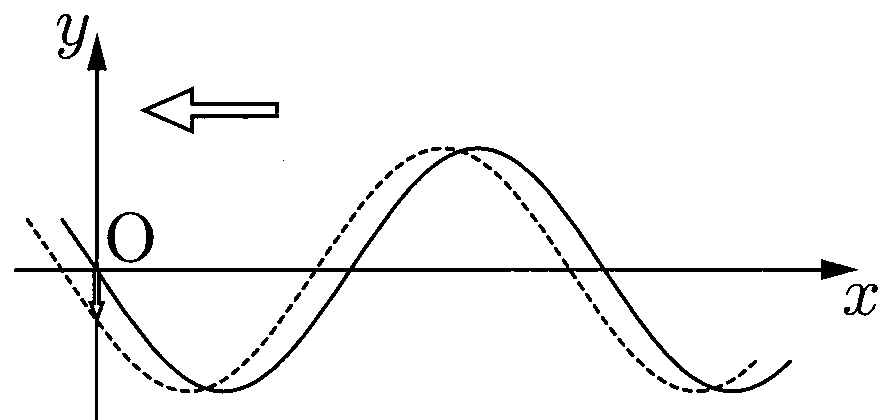
\includegraphics[keepaspectratio,width=62mm]{fig/n14_a6_2a.png}\end{center}
       よって，次の瞬間，原点の媒質は$-y$の向きに動き出すと分かる．振幅$A\U{m}$，周期$T\U{s}$，時刻$t=0\U{s}$における変位が$y=0\U{m}$で$-y$の向きに動き出す単振動という条件を満たす単振動の時間変動のグラフは次の$y-t$グラフのようなものに限られる．
       \begin{center}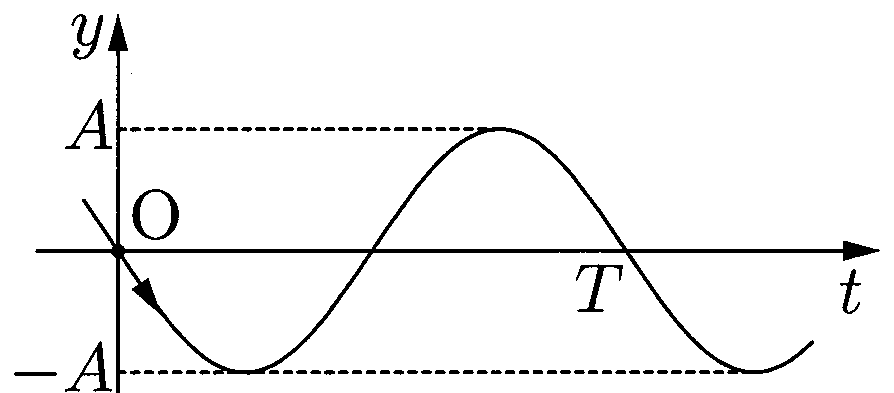
\includegraphics[keepaspectratio,width=62mm]{fig/n14_a6_2b.png}\end{center}
       これを数式化すると，
       \[y(0,t)=-A\sin 2\pi\frac{t}{T}\U{m}\Ans\]
\ko{3} 与えられた$y-x$グラフに代表値をつけると以下のようになる．
       \begin{center}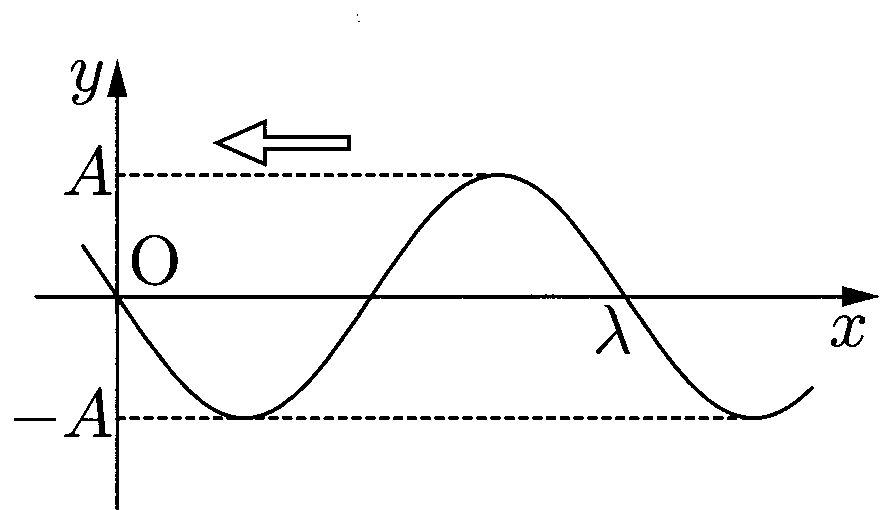
\includegraphics[keepaspectratio,width=62mm]{fig/n14_a6_3a.png}\end{center}
       よって，時刻$t=0\U{s}$の波形を数式化すると，
       \[y(x,0)=-A\sin 2\pi\frac{x}{\lambda}\U{m}\]
       である．波の進行する速さは，
       \[v=f\lambda=\frac{1}{T}\cdot\lambda\U{m/s}\]
       であり，負の向きに波が進んでいることに注意すると，時刻$t\U{s}$に位置$x\U{m}$に存在する波は，時刻$t=0\U{s}$においては$x+\dfrac{\lambda}{T}t\U{m}$の位置にいたはずである．
       \begin{center}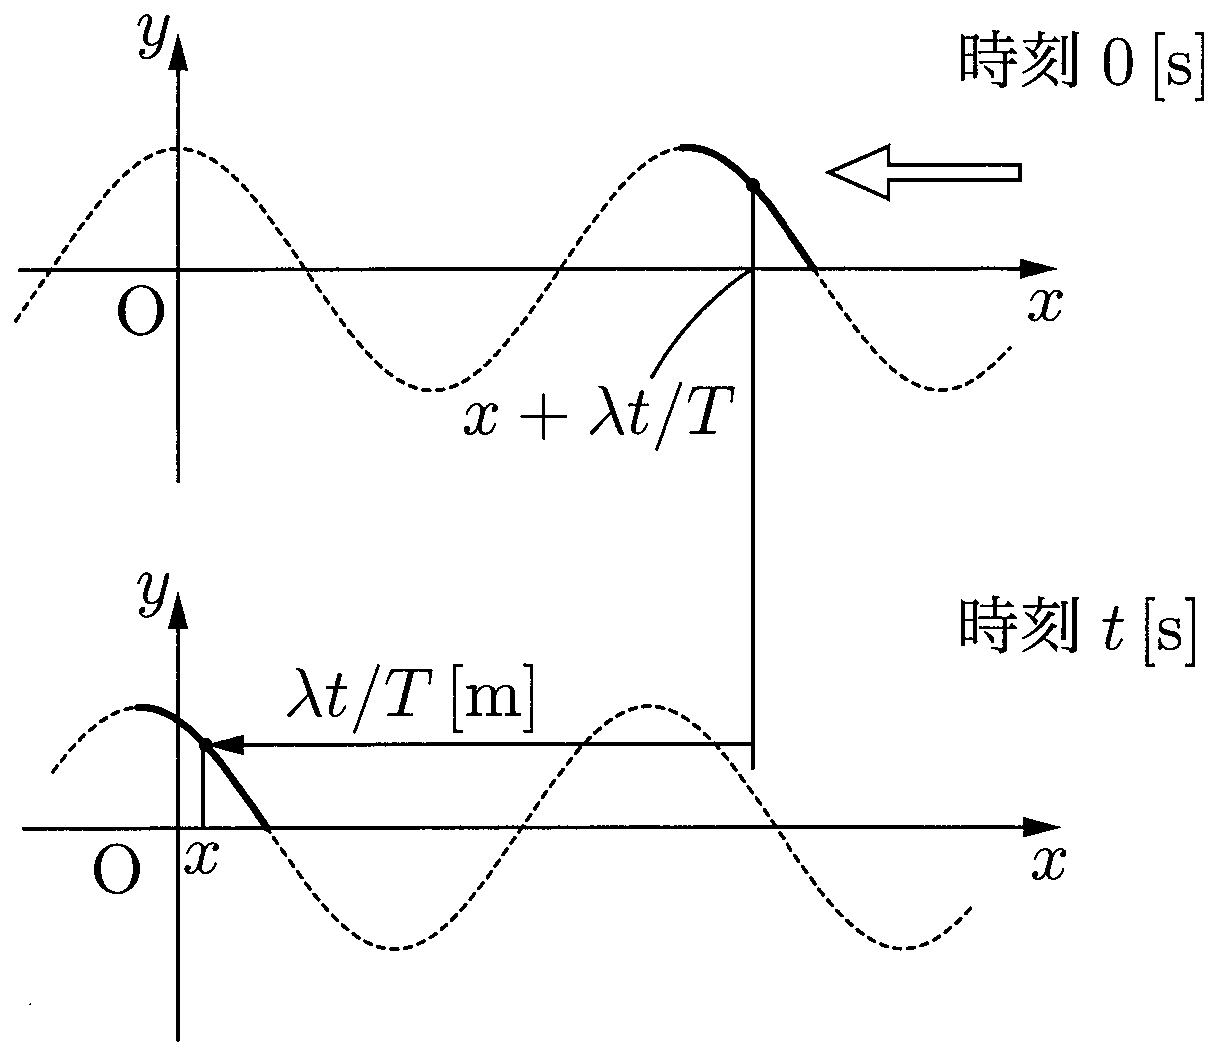
\includegraphics[keepaspectratio,width=62mm]{fig/n14_a6_3b.png}\end{center}
       よって，
       \[y(x,t)=y\left(x+\frac{\lambda}{T}t,\,0\right)\]
       \[=-A\sin 2\pi\frac{x+\lambda t/T}{\lambda}\]
       \[=-A\sin 2\pi\left(\frac{x}{\lambda}+\frac{t}{T}\right)\U{m}\]
       これに$x=0\U{m}$を代入すると，
       \[y(0,t)=-A\sin 2\pi\frac{t}{T}\U{m}\]
       となり，確かに(2)の答えと一致する．\hspace*{\fill}\Ans
\end{komon}
\begin{chuu}
(3)の問題の場合は，一般表式を経由して得られた答えと(2)の答えが完全に一致したが，見かけ上，異なる式として得られる場合もあるので注意せよ．例えば(1)について同様な計算を行うと，
\[y(x,t)=y\left(x-\frac{\lambda}{T}t,\,0\right)=-A\sin 2\pi\frac{x-\lambda t/T}{\lambda}\]
\[=-A\sin 2\pi\left(\frac{x}{\lambda}-\frac{t}{T}\right)\U{m}\]
となり，これに$x=0\U{m}$を代入すると，
\[y(0,t)=-A\sin\left(-2\pi\frac{t}{T}\right)\U{m}\]
となり，(1)の$y(0,t)=A\sin 2\pi\dfrac{t}{T}\U{m}$とは見かけ上異なるが，この2式が同一のものであるのは明らかである．このように，求め方によっては三角関数の中味の部分の正負が逆の表式として得られることもあるが，数学的には必ず等価な式になる．
\end{chuu}

\MonN{7}{縦波の横波表示}\par\nopagebreak
\begin{sisin}
横波表示した縦波について媒質の変位を考えるには，$+y$の向きの変位を$+x$の向きの変位に戻せばよいので，グラフの各点を平衡点を中心に{\gtfamily 時計回りに90度回転}すればよい．その図を元にすれば，疎密も容易に判定ができるだろう．

媒質の速さをいきなり考えるのは難しいので，まず横波と同様に次の瞬間の波形を作図し，横波表示の場合には媒質が次の瞬間にどちら向き（$+y$もしくは$-y$）に動くのかを考える．もし横波表示の場合に$+y$の向きに動くのであれば，媒質は$+x$の向きに動くと考えられる（$+x$の向きの変位を$+y$の向きに取り直して横波表示しているから）．
\end{sisin}
\KaiHead
\begin{komon}
\ko{1} 媒質の変位を時計回りに90度回転させればよいので，図の通りである．
       \begin{center}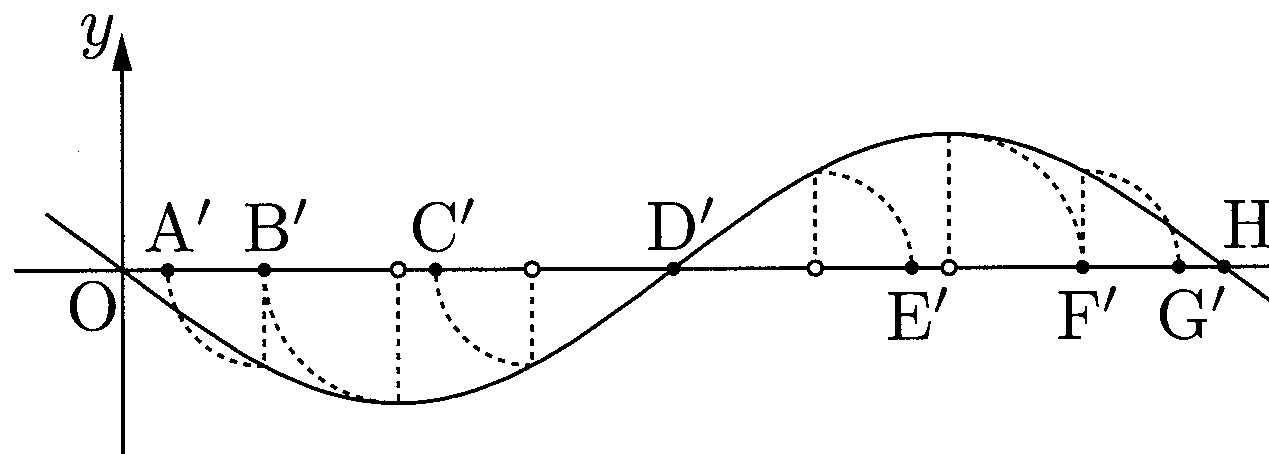
\includegraphics[keepaspectratio,width=62mm]{fig/n14_a7_disp.png}\end{center}
\end{komon}
\begin{chuu}
例えば変位したあとの$\mathrm{F}$点が$\mathrm{G}$点に重なっているが，特に問題はない（もともと$\mathrm{G}$点にいた媒質は$\mathrm{G}^\prime$点に移動しているので，媒質は重なってはいない）．
\end{chuu}
\begin{komon}
\ko{2} (1)の結果より，$\mathrm{H}$点には左右から媒質が集まってきている．よって，媒質の密度が最大であるのは，点$\mathrm{H}$である．\hspace*{\fill}\Ans

       また，$\mathrm{D}$点の回りの媒質は$\mathrm{D}$点から遠ざかる向きに逃げているので，媒質の密度が最小であるのは，点$\mathrm{D}$である．\hspace*{\fill}\Ans
\ko{3} 横波表示のままで次の瞬間の波形を描いてみると，次図の破線のようになる．
       \begin{center}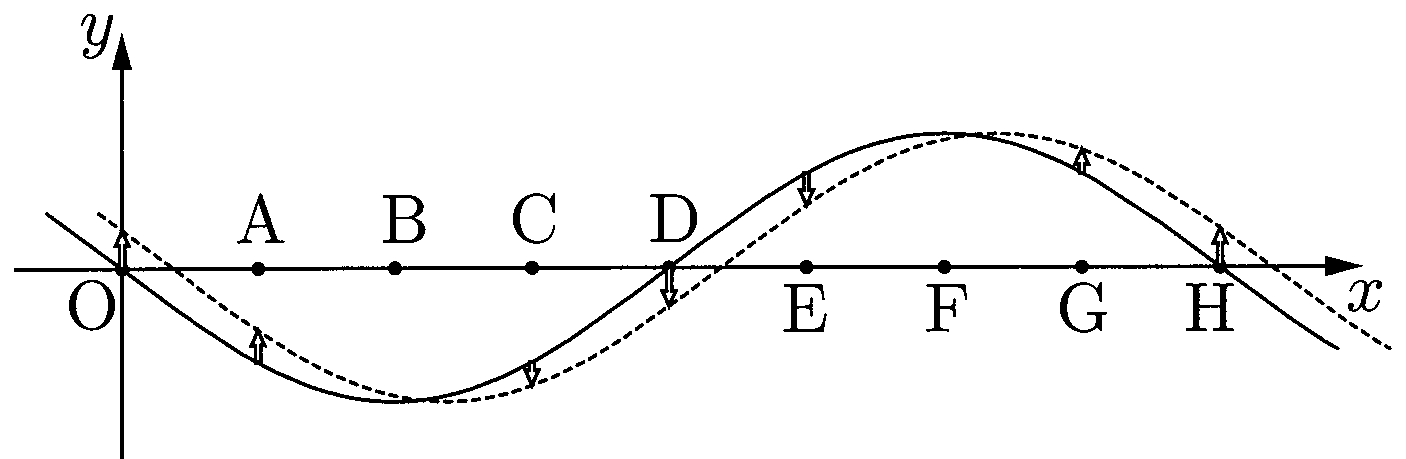
\includegraphics[keepaspectratio,width=62mm]{fig/n14_a7_yoko.png}\end{center}
       よって，この瞬間における各媒質の移動の向きは，横波表示で考えると，$\mathrm{A}:\uparrow$, $\mathrm{B}$：なし, $\mathrm{C}:\downarrow$, $\mathrm{D}:\downarrow$, $\mathrm{E}:\downarrow$, $\mathrm{F}$：なし, $\mathrm{G}:\uparrow$, $\mathrm{H}:\uparrow$となっている．これを時計まわりに$90^\circ$回転させて実際の縦波の媒質の移動に戻すと，次図のようになる．
       \begin{center}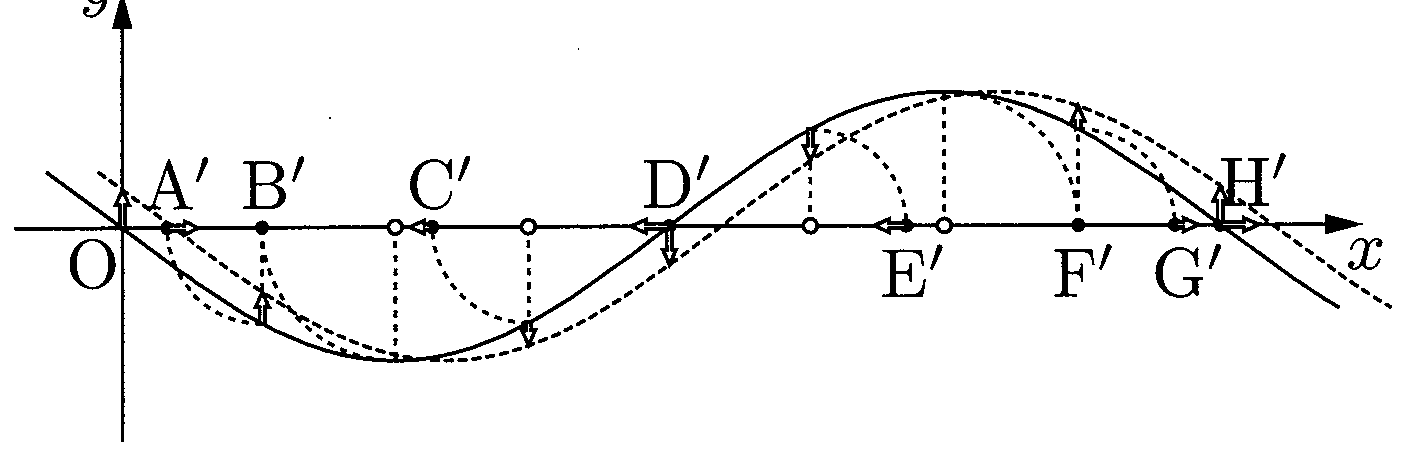
\includegraphics[keepaspectratio,width=62mm]{fig/n14_a7_jissai.png}\end{center}
       よって，この瞬間における各媒質の実際の移動の向きは，それぞれ$\mathrm{A}:\Rightarrow$, $\mathrm{B}$：なし, $\mathrm{C}:\Leftarrow$, $\mathrm{D}:\Leftarrow$, $\mathrm{E}:\Leftarrow$, $\mathrm{F}$：なし, $\mathrm{G}:\Rightarrow$, $\mathrm{H}:\Rightarrow$となる．

       ここで媒質の速さが最大となるのは，単振動の中心である$\mathrm{D}$, $\mathrm{H}$点であるから，
       \[\text{速さが}+x\text{の向きに最大となる位置：点}\mathrm{H}\]
       \[-x\text{の向きに最大となる位置：点}\mathrm{D}\Ans\]
\end{komon}

\Rank{C問題}
\MonN{8}{波動の表式}\par\nopagebreak
\begin{sisin}
波動の進行現象とは，同じ変位を与える点が，時刻$t\U{s}$の進行とともに$x$軸正の向きもしくは負の向きに移動していくものである．同じ変位を与えるためには位相が等しければよいので，位相$bt-cx$について，時刻$t\U{s}$が増加したときに同じ位相値を与える$x$座標が増えるかどうかを考えれば波の進行の向きが分かる．

波動の表式から波の振幅，波長，周期を求めるためには，時刻$t\U{s}$もしくは位置$x\U{m}$を固定し（定数だとみなす），そして波長，周期などの意味を考えてこれらを表式から得ればよい．

また，残りの振動数，伝播速度は，$f=\dfrac{1}{T}$, $vT=\lambda$などの関係式を用いて求める．
\end{sisin}
\KaiHead
\begin{komon}
\ko{1} 波が進むとは，{\gtfamily 同じ変位を与える点（＝位相が等しい点）が時間とともに移動していく}ことである．したがって，位相$bt-cx$の値を一定に保つには$x$がどう変化しなければならないかを調べればよい．

       $t$が増えると$bt$が増えるので，$bt-cx$を一定に保つには$cx$も同じだけ増えなければならない．すなわち$x$が増加しなければならない．よって同じ位相の点は時刻の進行とともに$x$軸正の向きへ移動していくので，この波の進行の向きは$x$軸正の向きである．\hspace*{\fill}\Ans
\end{komon}
\begin{bekkai}
分かりにくければ，具体的な数値を当てはめて考えてしまうとよい．例えば変位が0となる点のひとつである，位相$bt-cx=0$の点について考えてみると，位相0を与える座標は
\[x=\frac{b}{c}t\U{m}\]
であるから，これは時刻$t\U{s}$の進行とともに$x$軸正の向きに移動していく．よって，この波の進行の向きは$x$軸正の向きである．
\end{bekkai}
\begin{bsHosoku}{参考}
以上のことをさらにまとめると，以下のようなことが導ける．位相部分（三角関数の中味）の$x$, $t$が同符号の場合，その式は$x$軸負の向きへと進む波を表す．逆に，$x$, $t$が異符号の場合，その式は$x$軸正の向きへと進む波を表す．
\end{bsHosoku}
\begin{komon}
\ko{2} 例えば時刻$t=t_0\U{s}$に着目すると，この時刻における波形は
       \[y(x,t_0)=a\sin(bt_0-cx)\U{m}\]
       で与えられ，$bt_0$が定数であることに注意すると，時刻$t=t_0\U{s}$における$y-x$グラフは次図のようになる．
       \begin{center}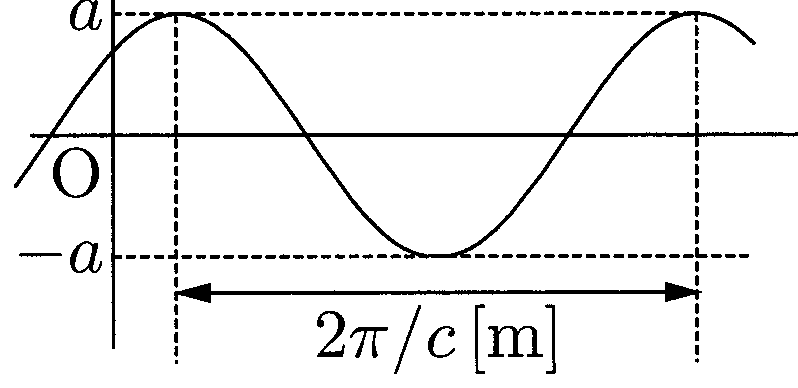
\includegraphics[keepaspectratio,width=62mm]{fig/n14_a8_yx.png}\end{center}
       よって，
       \[\text{振幅}\ A=a\U{m},\hspace{4mm}\text{波長}\ \lambda=\frac{2\pi}{c}\U{m}\Ans\]
\end{komon}
\begin{chuu}
$y(x,t_0)=a\sin(bt_0-cx)\U{m}$の繰り返し単位が$\dfrac{2\pi}{c}\U{m}$になることは次のように考えれば分かる．座標$x$が1波長$\lambda\U{m}$だけずれると位相部分$bt_0-cx$が$2\pi$ずれるので，
\[bt_0-c(x+\lambda)=bt_0-cx-2\pi\]
である．よって，繰り返し周期$\lambda\U{m}$は
\[\lambda=\frac{2\pi}{c}\U{m}\]
となる．
\end{chuu}
\begin{bekkai}
上述の解答が分かりにくい人は，もっと具体的な値を代入して考えるとよいだろう．例えば，時刻$t=0\U{s}$における位置$x\U{m}$の変位$y(x,0)\U{m}$を考えると，
\[y(x,0)=a\sin(b\cdot 0-cx)=-a\sin cx\U{m}\]
となるので，周期を考えれば$\lambda=\dfrac{2\pi}{c}\U{m}$が分かる．
\end{bekkai}
\hspace{1zw}次に，例えば座標$x=x_0\U{m}$に着目すると，この位置における単振動は
\[y(x_0,t)=a\sin(bt-cx_0)\U{m}\]
で与えられ，$cx_0$が定数であることに注意すると，座標$x=x_0\U{m}$における$y-t$グラフは次図のようになる．
\begin{center}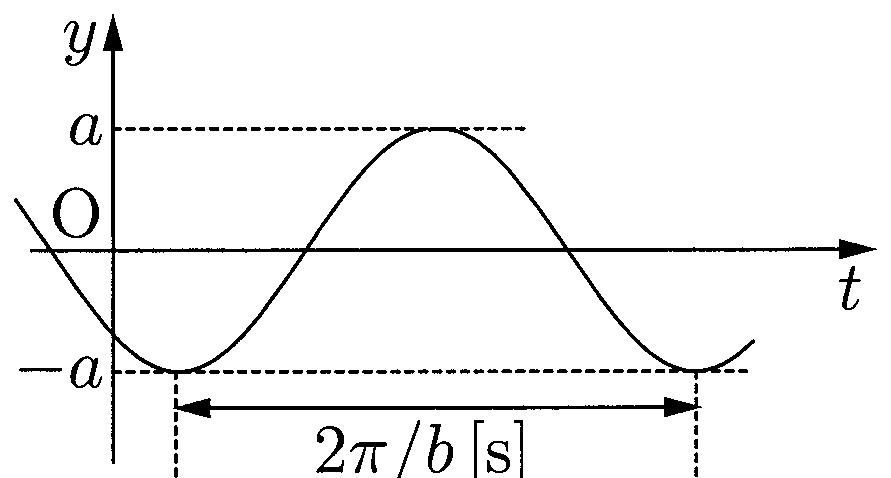
\includegraphics[keepaspectratio,width=62mm]{fig/n14_a8_yt.png}\end{center}
\hspace{1zw}よって，この点の単振動の周期（＝波動の周期）は
\[T=\frac{2\pi}{b}\U{s}\Ans\]
\begin{bekkai}
これも同様にもっと具体的な値を代入して考えてもよい．例えば原点$x=0\U{m}$における時刻$t\U{s}$の変位$y(0,t)\U{m}$は，
\[y(0,t)=a\sin(b\cdot t-c\cdot 0)=a\sin bt\U{m}\]
で与えられるので，これをグラフ化して振動周期を得てもよい．
\end{bekkai}
\hspace{1zw}以上を用いて波の振動数および伝播速度を求めると，
\[f=\frac{1}{T}=\frac{1}{2\pi/b}=\frac{b}{2\pi}\U{Hz}\Ans\]
\[v=f\lambda=\frac{b}{c}\U{m/s}\Ans\]
\begin{bsHosoku}{参考}
波の伝播速度については，(1)の別解で考えた，同位相の点がどの座標に移動していくのかによって考えることも可能である．例えば，位相が$\varphi_0\U{rad}$となる点が時刻とともにどの位置に移動していくのかを考えると，
\[x=\frac{bt-\varphi_0}{c}\U{m}\]
であるので，その移動速度は
\[\frac{dx}{dt}=\frac{b}{c}\U{m/s}\]
となる．これから分かるように，一般に波の速さと呼ばれているものは，波の同位相の点（＝同変位の点）がどれだけの速度で動いていくかを表すものであり，これを{\gtfamily 位相速度}と呼ぶ．

一方，媒質は上下に単振動をしているのみであり，この媒質が動いている速度については$\dfrac{d}{dt}y(x,t)$で与えられる．
\end{bsHosoku}

\MonN{9}{波の位相}\par\nopagebreak
\begin{sisin}
正弦波の表式における三角関数の角度部分のことを位相というが，この位相に着目して考えると位置のずれと時間のずれとを一括して同様に扱うことができるというメリットがある．位相という概念そのものは本質的には非常に難しいのだが，高校範囲では特に以下のことを覚えておけば十分である．

ある時刻において，位置が一波長分ずれていると位相は$2\pi$ずれている．

同じ位置において，時刻が一周期分ずれていると位相は$2\pi$ずれている．

位相の差が，$2\pi$の整数倍になっているような二つの位相を，互いに同位相であるといい，このとき二つの変位は等しくなっている．

位相の差が，$2\pi$の整数倍$+\pi$になっているような二つの位相を，互いに逆位相であるといい，このとき二つの変位はちょうど正負逆になっている．
\end{sisin}
\KaiHead
\begin{komon}
\ko{1} 位置$\mathrm{A}$と位置$\mathrm{B}$はちょうど$\dfrac{1}{4}$波長分だけ位置がずれているので，ある時刻に着目すると，位置$\mathrm{A}$と位置$\mathrm{B}$は必ず$\dfrac{1}{4}$波長分だけずれた変位を持っている．これを位相に換算すると，位置の1波長分ずれは位相の$2\pi$のずれに相当するので，
       \[\Delta\varphi=2\pi\times\frac{1}{4}=\frac{\pi}{2}\U{rad}\Ans\]
\ko{2} 互いに同位相であるとき，二つの位相の差は$2\pi$の整数倍となっているが，位相の$2\pi$分のずれは位置の1波長分のずれに相当するから，$\mathrm{A}$点と同位相の点とは$\mathrm{A}$点から整数波長分だけ離れた点であると言える．よって，位置$\mathrm{A}$と同位相の位置は図より$\mathrm{E}$点．\hspace*{\fill}\Ans
% 原本は(3)の結論を「位置Aと同位相の位置は図よりC, G点」と書いているが，(3)は逆位相を問うて
% いるので「逆位相の位置」の誤り（明らかな誤植）．ここでは訂正して転記した．
\ko{3} 互いに逆位相であるとき，二つの位相の差は$2\pi$の整数倍$+\pi$となっているから，$\mathrm{A}$点と逆位相の点とは$\mathrm{A}$点から整数波長分＋半波長分だけ離れた点であると言える．よって，位置$\mathrm{A}$と逆位相の位置は図より$\mathrm{C}$, $\mathrm{G}$点．\hspace*{\fill}\Ans
\end{komon}
\begin{chuu}
互いに同位相である点の変位は等しくなっているが，変位が等しいからといって同位相であるとは限らないことに注意．(2)のように変位が0となる点同士でも$\mathrm{A}$と$\mathrm{C}$は逆位相であるし，また例えば$\mathrm{A}$, $\mathrm{B}$の中点と$\mathrm{B}$, $\mathrm{C}$の中点の変位は同じであるがこれらは同位相の点でも逆位相の点でもない．
\end{chuu}
\begin{bsHosoku}{参考}
「$\mathrm{A}$点の位相$\varphi_\mathrm{A}$に対して$\mathrm{B}$点の位相$\varphi_\mathrm{B}$の方が$\dfrac{\pi}{2}\U{rad}$だけ位相が進んでいる」とは，$\varphi_\mathrm{A}$と$\varphi_\mathrm{B}$の関係式が
\[\varphi_\mathrm{B}=\varphi_\mathrm{A}+\frac{\pi}{2}\U{rad}\]
となっていることを意味する．遅れている場合は
\[\varphi_\mathrm{B}=\varphi_\mathrm{A}-\frac{\pi}{2}\U{rad}\]
となる．

例えば本問の場合，$\mathrm{B}$点に到達する波は，$\mathrm{A}$点に到達している波よりも常に$\dfrac{1}{4}$波長だけ先行している波である．このことを位相の関係で表現すると，「$\mathrm{A}$点の位相$\varphi_\mathrm{A}$に対して$\mathrm{B}$点の位相$\varphi_\mathrm{B}$の方が$\dfrac{\pi}{2}\U{rad}$だけ位相が進んでいる」となる．

同じことを時刻で考えると次のように言える．$\mathrm{B}$点には，$\mathrm{A}$点に到達するよりも常に$\dfrac{1}{4}$周期だけ先行して波が到達している．1周期のずれが$2\pi\U{rad}$のずれに相当することを利用すれば，$\dfrac{1}{4}$周期だけ先行するというのは位相が$\dfrac{\pi}{2}\U{rad}$だけ進んでいることに対応するので，このことを位相の関係で表現すると，「$\mathrm{A}$点の位相$\varphi_\mathrm{A}$に対して$\mathrm{B}$点の位相$\varphi_\mathrm{B}$の方が$\dfrac{\pi}{2}\U{rad}$だけ位相が進んでいる」と言うことができることになる．

すなわち，位置がずれているということも到達時刻がずれているということも，いずれも結局は「位相のずれ」を与える原因として考えることができ，位相のずれに直して考えればこの二つを一括して捉えることができるというメリットがある．実際，この進行波の表式は$y(x,t)=A\sin 2\pi\left(\dfrac{x}{\lambda}-\dfrac{t}{T}\right)\U{m}$の形で与えられるが，時刻$t\U{s}$における$\mathrm{A}$点の振動$y(0,t)$と$\mathrm{B}$点の振動$y\left(\dfrac{\lambda}{4},t\right)$，および時刻$t\U{s}$に$\mathrm{B}$点にやってくる波が$\mathrm{A}$点を通過する瞬間の振動$y\left(0,t-\dfrac{1}{4}T\right)$の三つを比較してみよ．いずれも位相の関係が「$\mathrm{A}$点の位相$\varphi_\mathrm{A}$に対して$\mathrm{B}$点の位相$\varphi_\mathrm{B}$の方が$\dfrac{\pi}{2}\U{rad}$だけ位相が進んでいる」となっているにすぎないことが分かるだろう．
\end{bsHosoku}

\MonN{10}{縦波と媒質の関係}\par\nopagebreak
\begin{sisin}
縦波ではあるが，横波表示にした場合の扱い方は横波と全く同じである．すなわち，$y-x$グラフから$y-t$グラフを作る場合には，少し波を進めてみてどちらの向きに媒質が動くのかを判定することで考える．波動の進行の向きについては，波動が右へ進む場合と左へ進む場合それぞれについて原点についての$y-t$グラフを作図してみればよい．片方しか図2のようにはならない．

波動が左の向きへと進行している場合であっても，{\gtfamily 媒質が密となるのは$x$座標の増加につれて}{\gtfamily $y>0$から$y<0$へ変化する点であり，}{\gtfamily 疎となるのは$x$座標の増加につれて}{\gtfamily $y<0$から$y>0$へ変化する点である}（横波表示を縦波の実際の変位に直してみれば，密・疎の位置は波動の進行の向きによらないことが分かるはず，やってみよ）．

{\gtfamily 縦波の疎密判定は}{\gtfamily $y-t$グラフから行うことはできない}．なぜなら，疎密は周辺の座標の媒質が寄ってくるか遠ざかるかによって決まるからであり，$y-t$グラフでは着目している一点の移動についてしか分からないからである．よって，ある時刻における疎密判定には必ずその瞬間における$y-x$グラフを作図してそれを用いること．
\end{sisin}
\KaiHead
\begin{komon}
\ko{1} この縦波が$+x$の向きに進行しているとすると，次の瞬間に原点は$-y$の向き（実際には$-x$の向き）に変位する（次図参照）．
       \begin{center}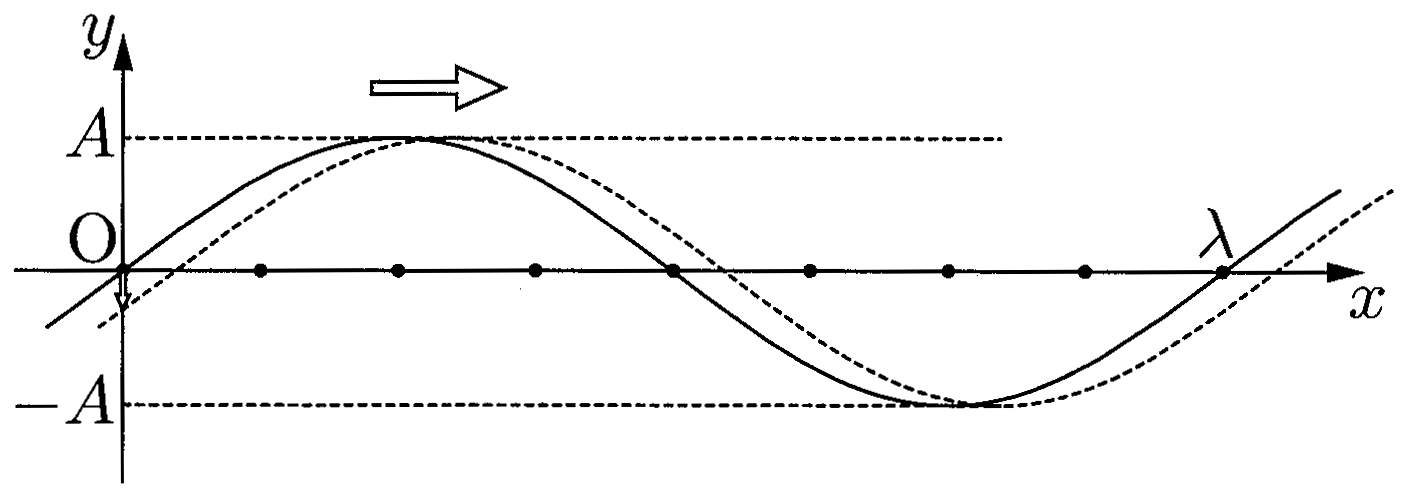
\includegraphics[keepaspectratio,width=62mm]{fig/n14_a10_p.png}\end{center}
       よって，これは図2のグラフに適合しない．一方，この縦波が$-x$の向きに進行しているとすると，次の瞬間に原点は$+y$の向き（実際には$+x$の向き）に変位する（次図参照）．
       \begin{center}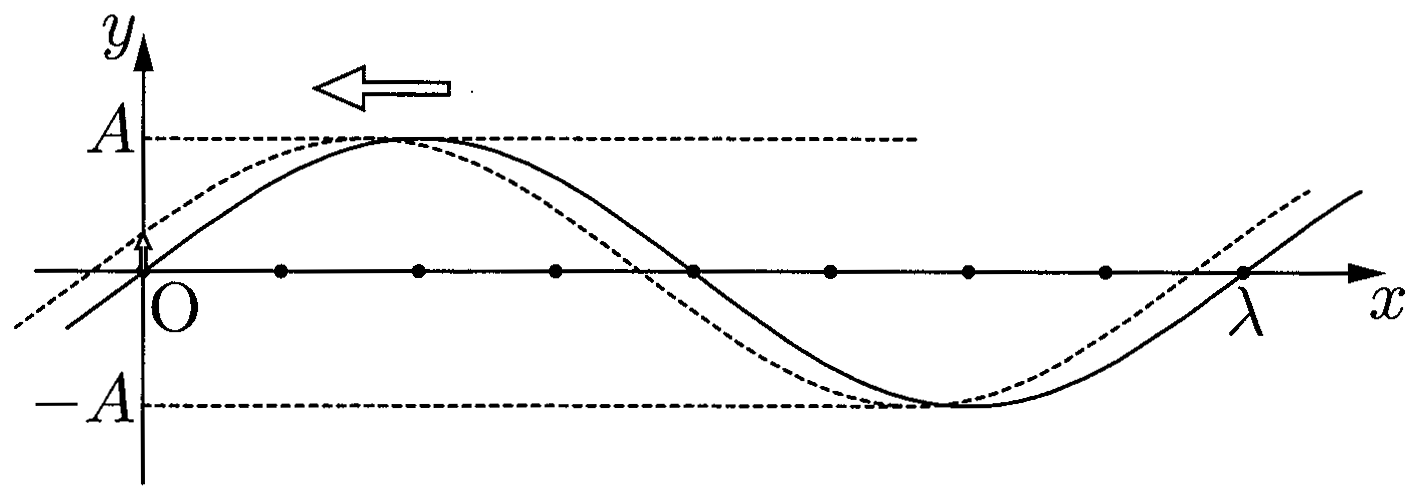
\includegraphics[keepaspectratio,width=62mm]{fig/n14_a10_m.png}\end{center}
       よって，これは図2のグラフに適合する．以上より，この縦波の進行の向きは$-x$の向きである．\hspace*{\fill}\Ans

       また，この縦波の波長は$\lambda\U{m}$，周期は$T\U{s}$であるから波の進行する速さは，
       \[v=f\cdot\lambda=\frac{\lambda}{T}\U{m/s}\Ans\]
\ko{2} $0\leqq t<T\U{s}$の範囲，ということは，波動が左の向きへ$0\sim1$波長分ずれた範囲内で考えよ，ということを意味する．

       この波動の密点とは，$x$座標の増加につれて$y>0$から$y<0$へ変化する点（時刻$t=0\U{s}$であれば$x=\dfrac{\lambda}{2}\U{m}$の点）であり，波動（波形）が左の向きへ移動していくと共に，この密点も左の向きへとずれていく．そして$x=\dfrac{\lambda}{8}\U{m}$が初めて密となるのは次の図のような場合である．
       \begin{center}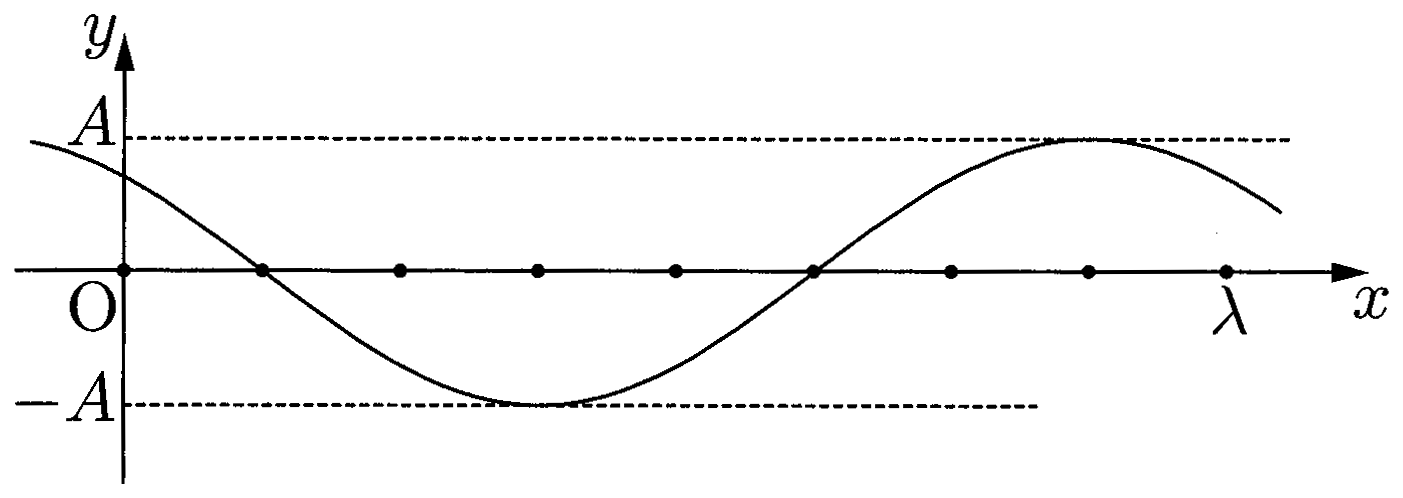
\includegraphics[keepaspectratio,width=62mm]{fig/n14_a10_dense.png}\end{center}
       また，この波形は，図1の状態から波形が左の向きへ$\dfrac{3}{8}\lambda\U{m}$だけ移動したものであるから，この状態になる時刻は，
       \[\frac{3}{8}T\U{s}\Ans\]
\end{komon}
\begin{chuu}
このときの媒質の実際の移動点を図示すると次図のようになる．波動の進行の向きが左の向きであっても，このとき$x=\dfrac{\lambda}{8}\U{m}$の点は確かに密点になっている．
\begin{center}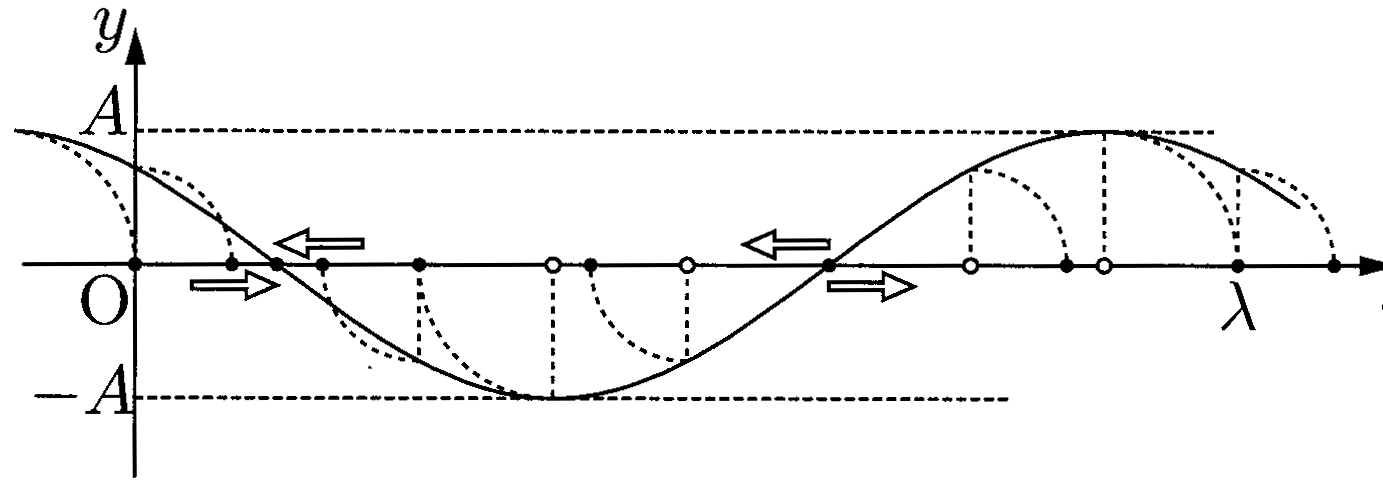
\includegraphics[keepaspectratio,width=62mm]{fig/n14_a10_chu.png}\end{center}
\end{chuu}
\begin{komon}
\ko{3} $t=\dfrac{3}{4}T\U{s}$のときには，波動は左の向きへ$\dfrac{3}{4}\lambda\U{m}$だけずれているので，このときの波形を図示すると次図のようになる．
       \begin{center}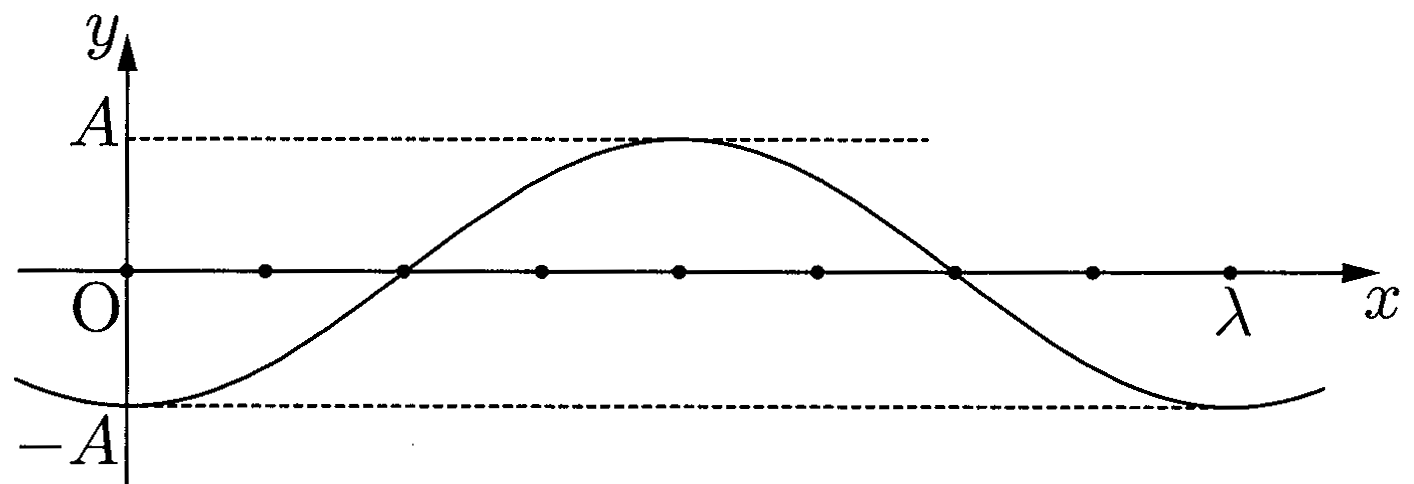
\includegraphics[keepaspectratio,width=62mm]{fig/n14_a10_34T.png}\end{center}
       よって，このときの密点は
       \[x=\frac{3}{4}\lambda\U{m}\Ans\]
\end{komon}

\end{multicols}
